\chapter{Интерфейс}\label{app:A}
\begin{figure}[h!]
    \centering
    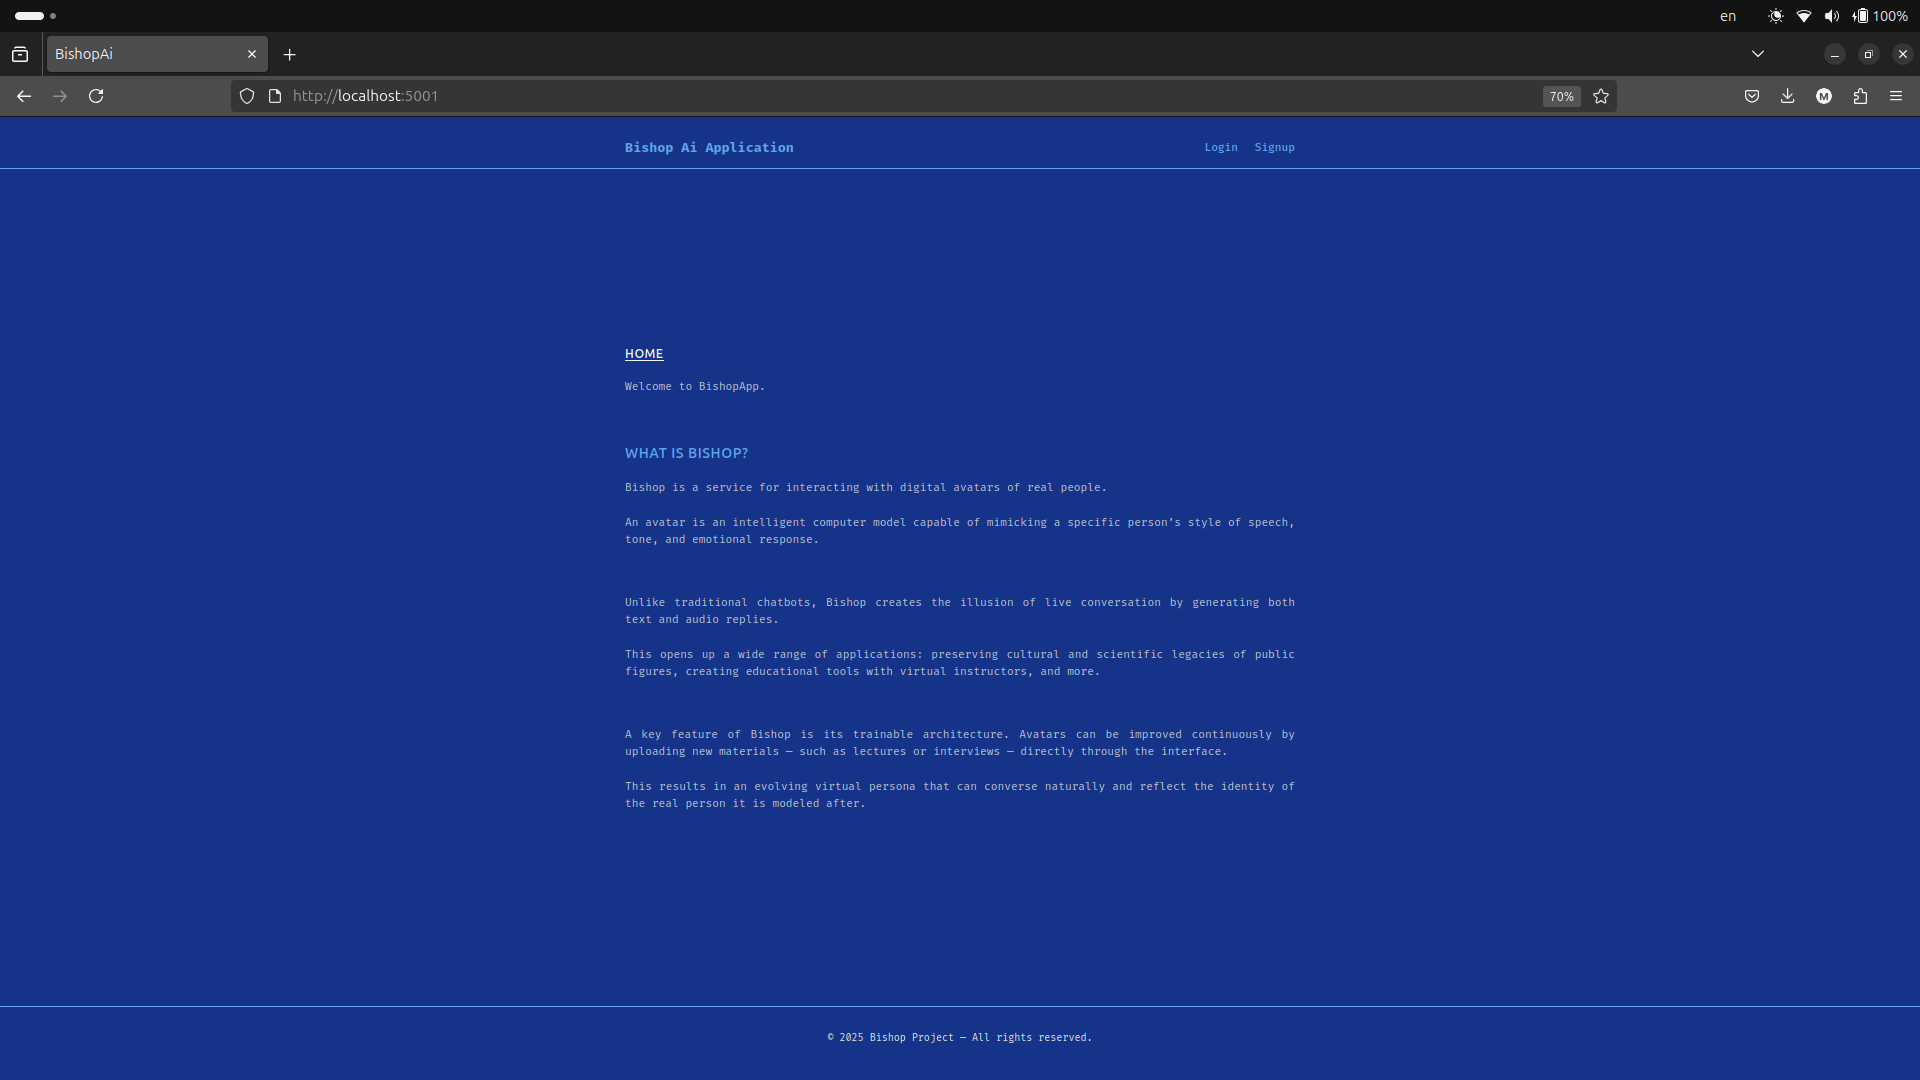
\includegraphics[width=1.0\linewidth]{images/ui/welcome.png}
    \caption{Гостевая страница}
    \label{fig:ui-page-welcome}
\end{figure}

\begin{figure}
    \centering
    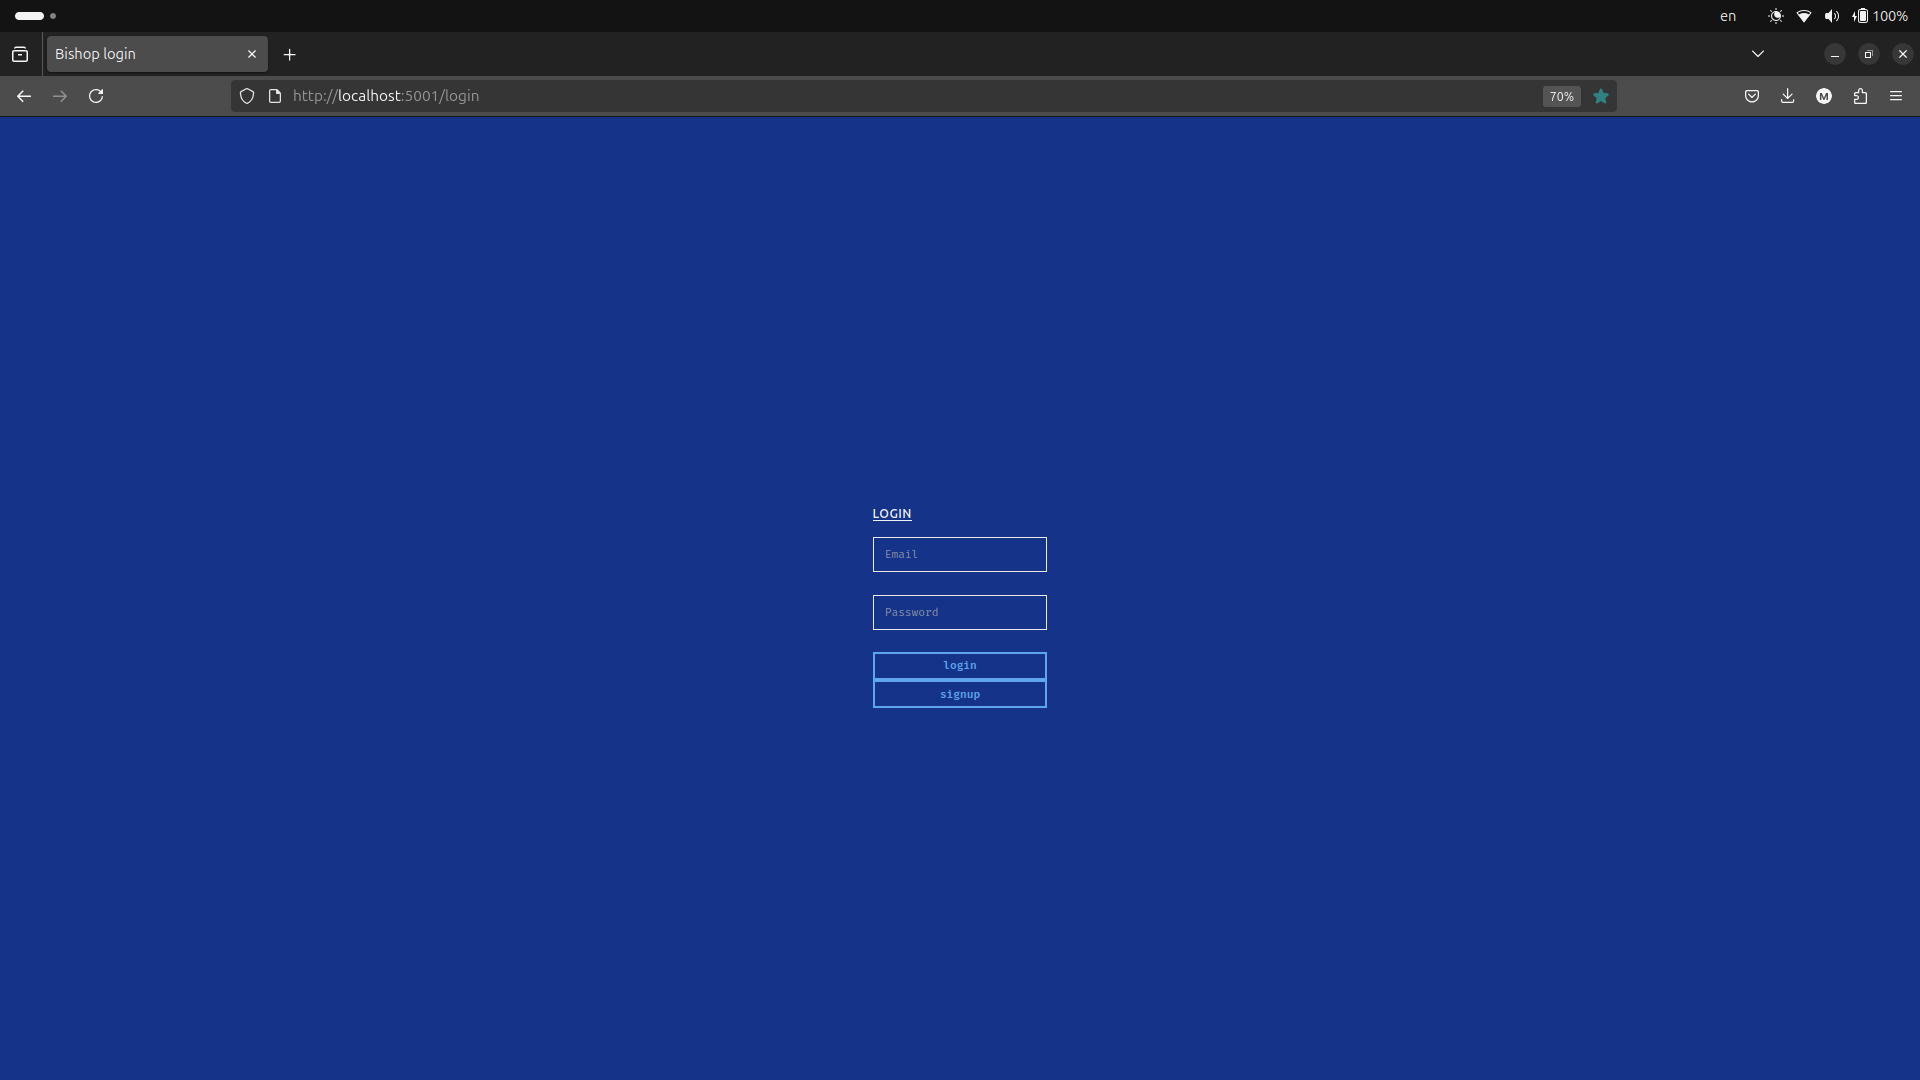
\includegraphics[width=1.0\linewidth]{images/ui/login.png}
    \caption{Страница аутентификации}
    \label{fig:ui-page-login}
\end{figure}

\begin{figure}
    \centering
    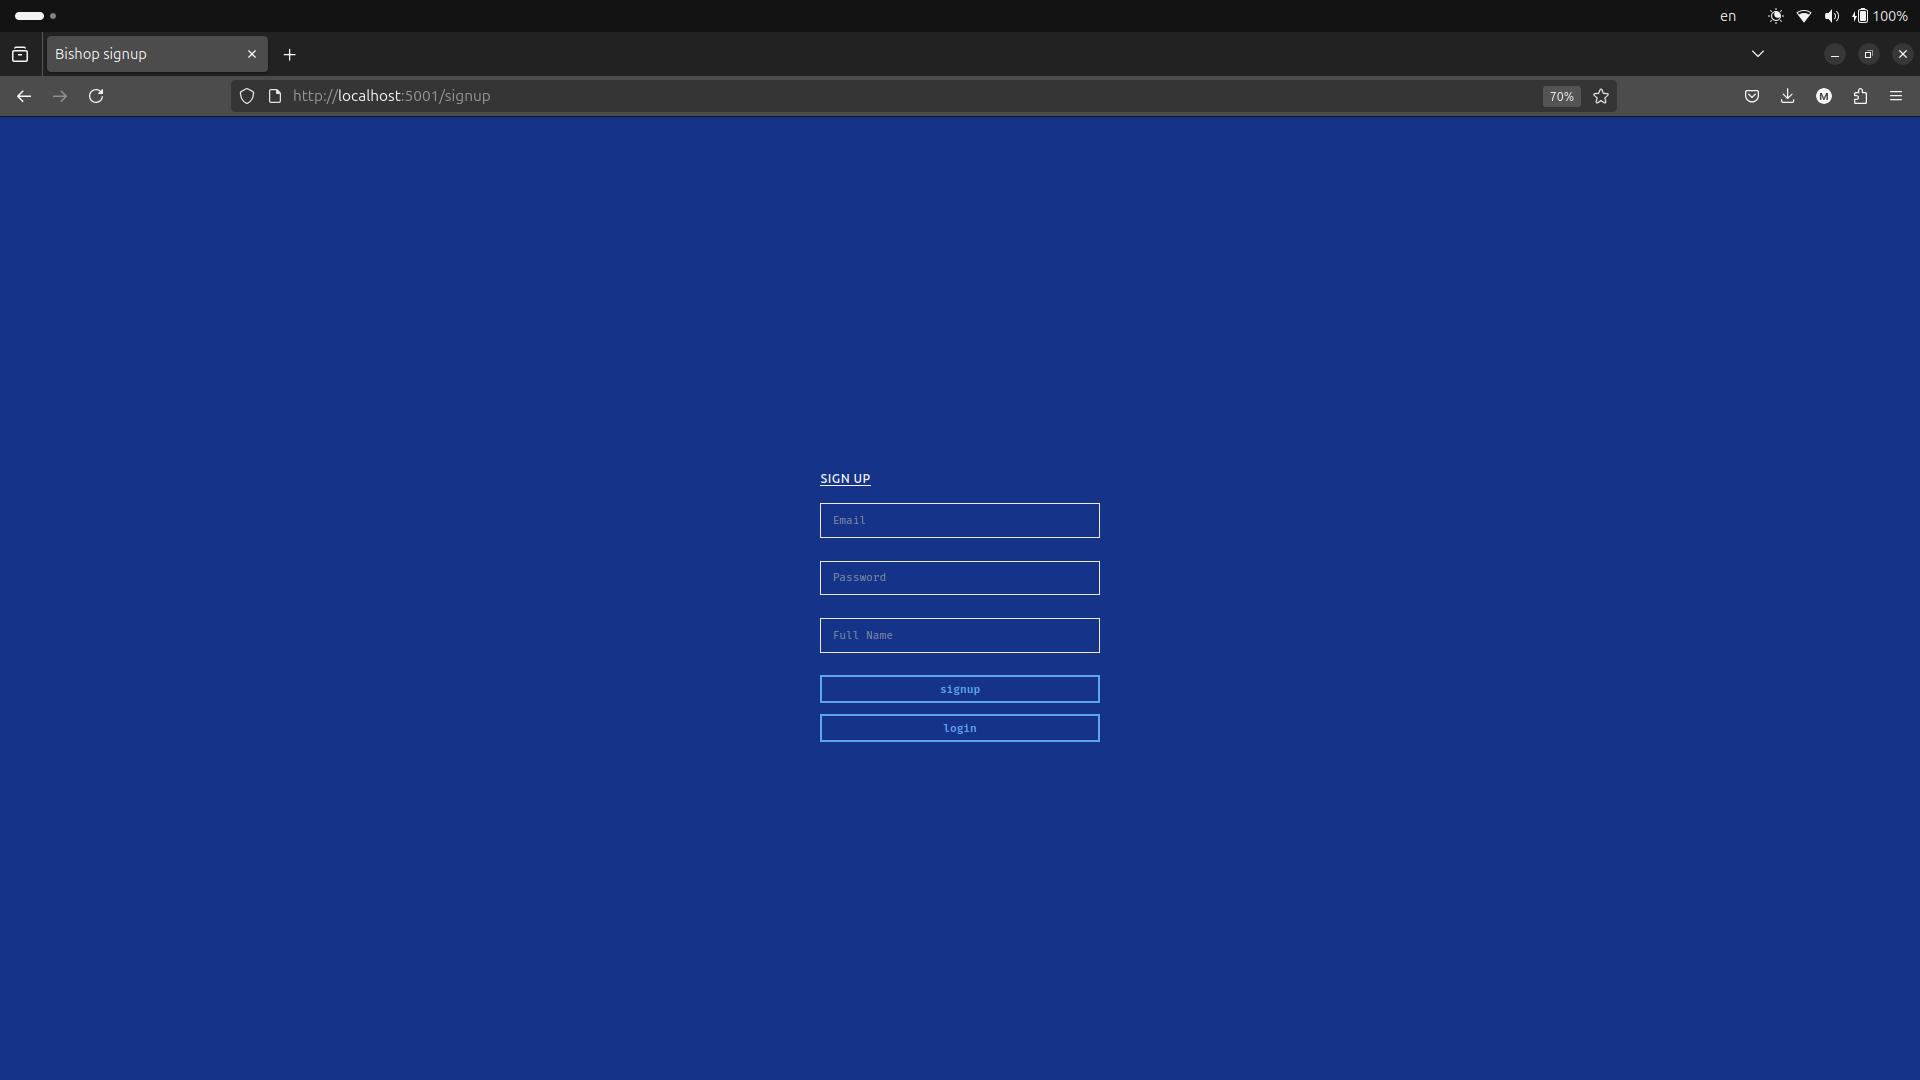
\includegraphics[width=1.0\linewidth]{images/ui/signup.png}
    \caption{Страница регистрации}
    \label{fig:ui-page-signup}
\end{figure}

\begin{figure}
    \centering
    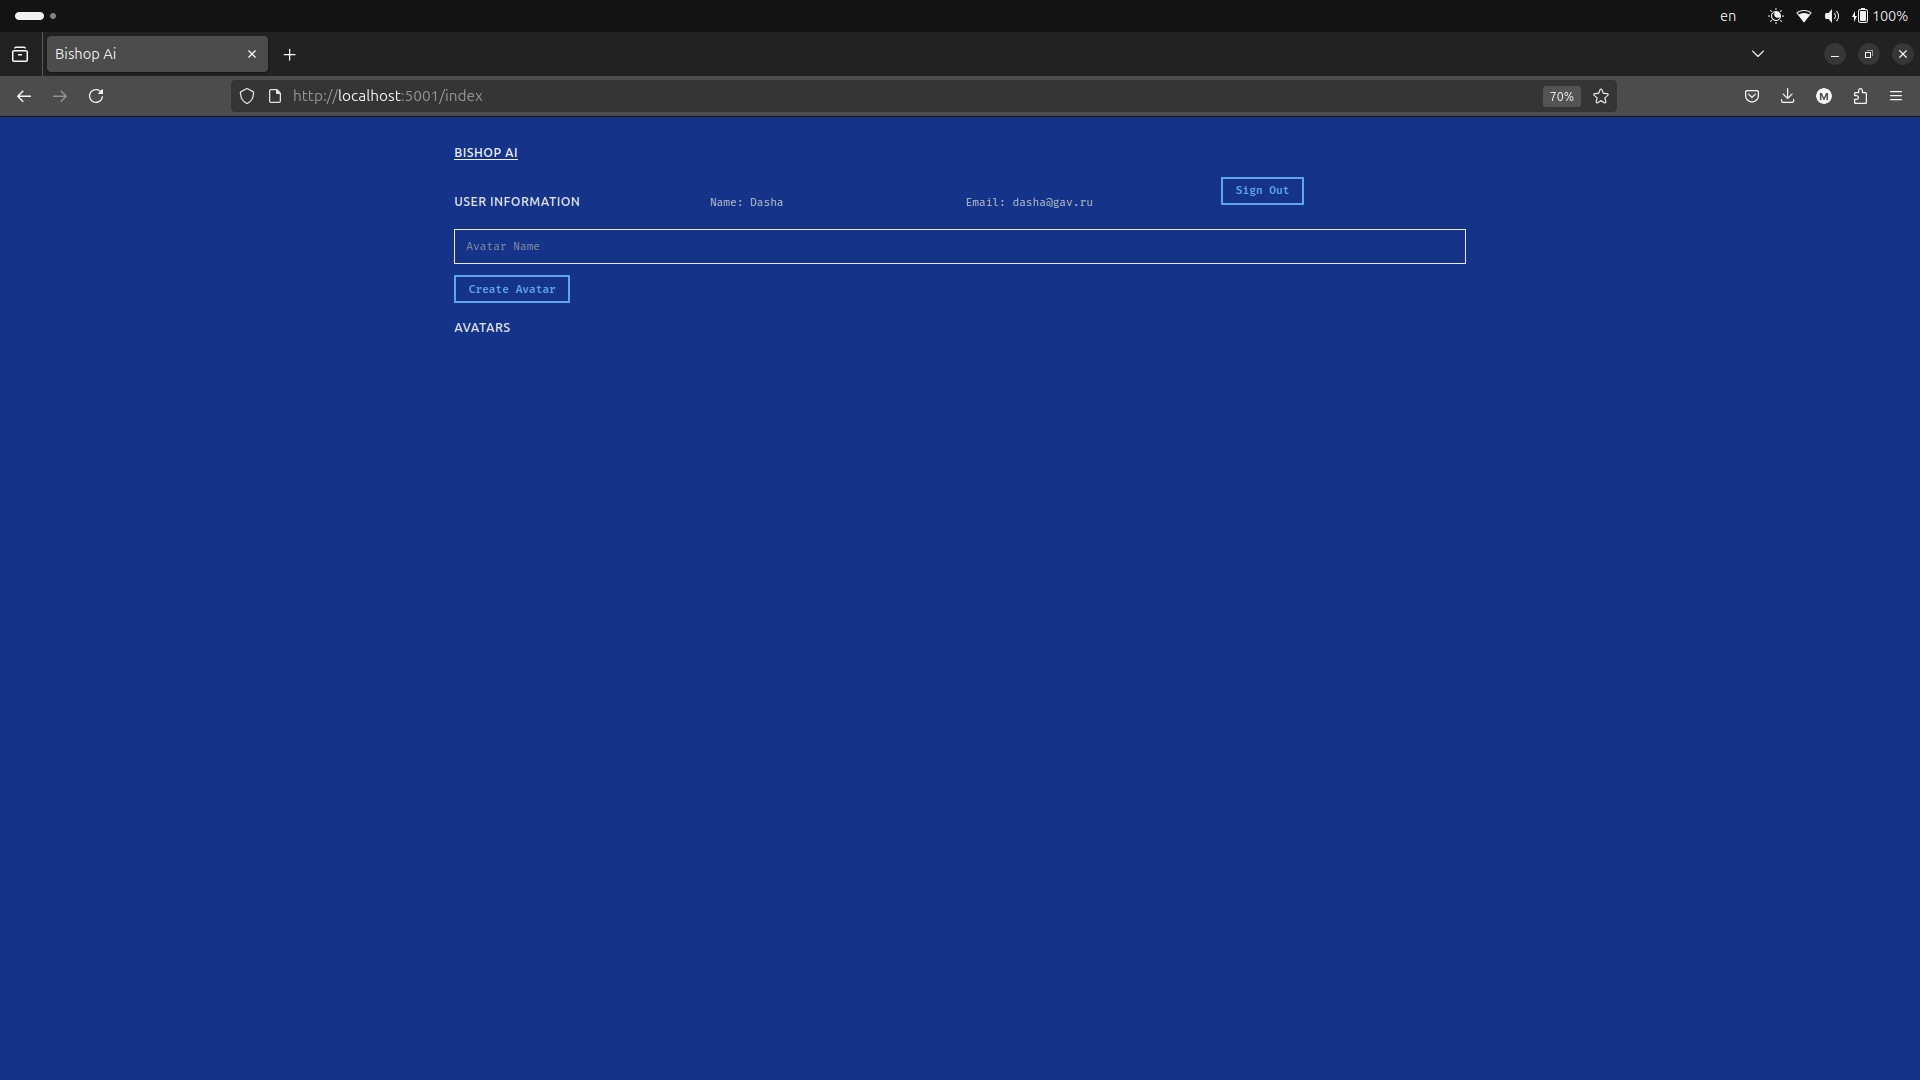
\includegraphics[width=1.0\linewidth]{images/ui/index.png}
    \caption{Основная страница приложения}
    \label{fig:ui-page-index}
\end{figure}

\begin{figure}
    \centering
    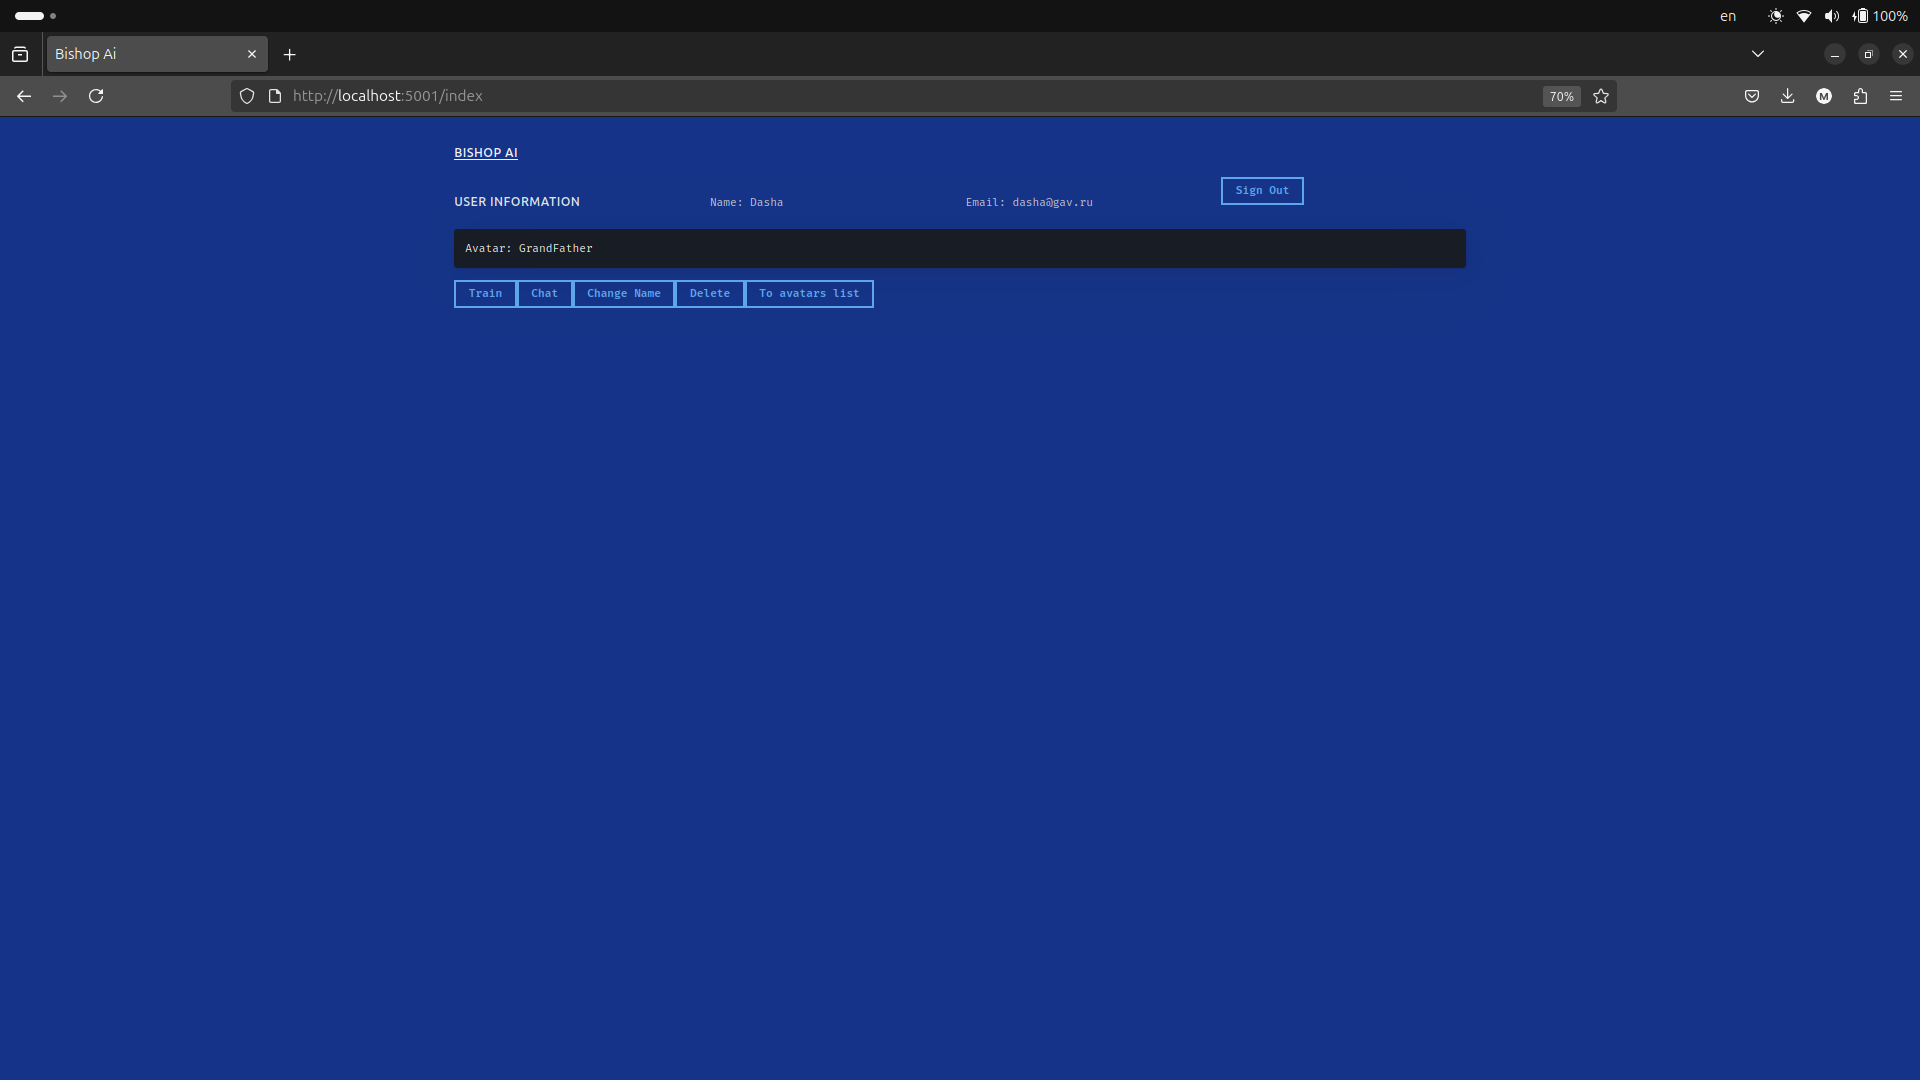
\includegraphics[width=1.0\linewidth]{images/ui/avatar.png}
    \caption{Страница управления аватарами}
    \label{fig:ui-page-avatar}
\end{figure}

\begin{figure}
    \centering
    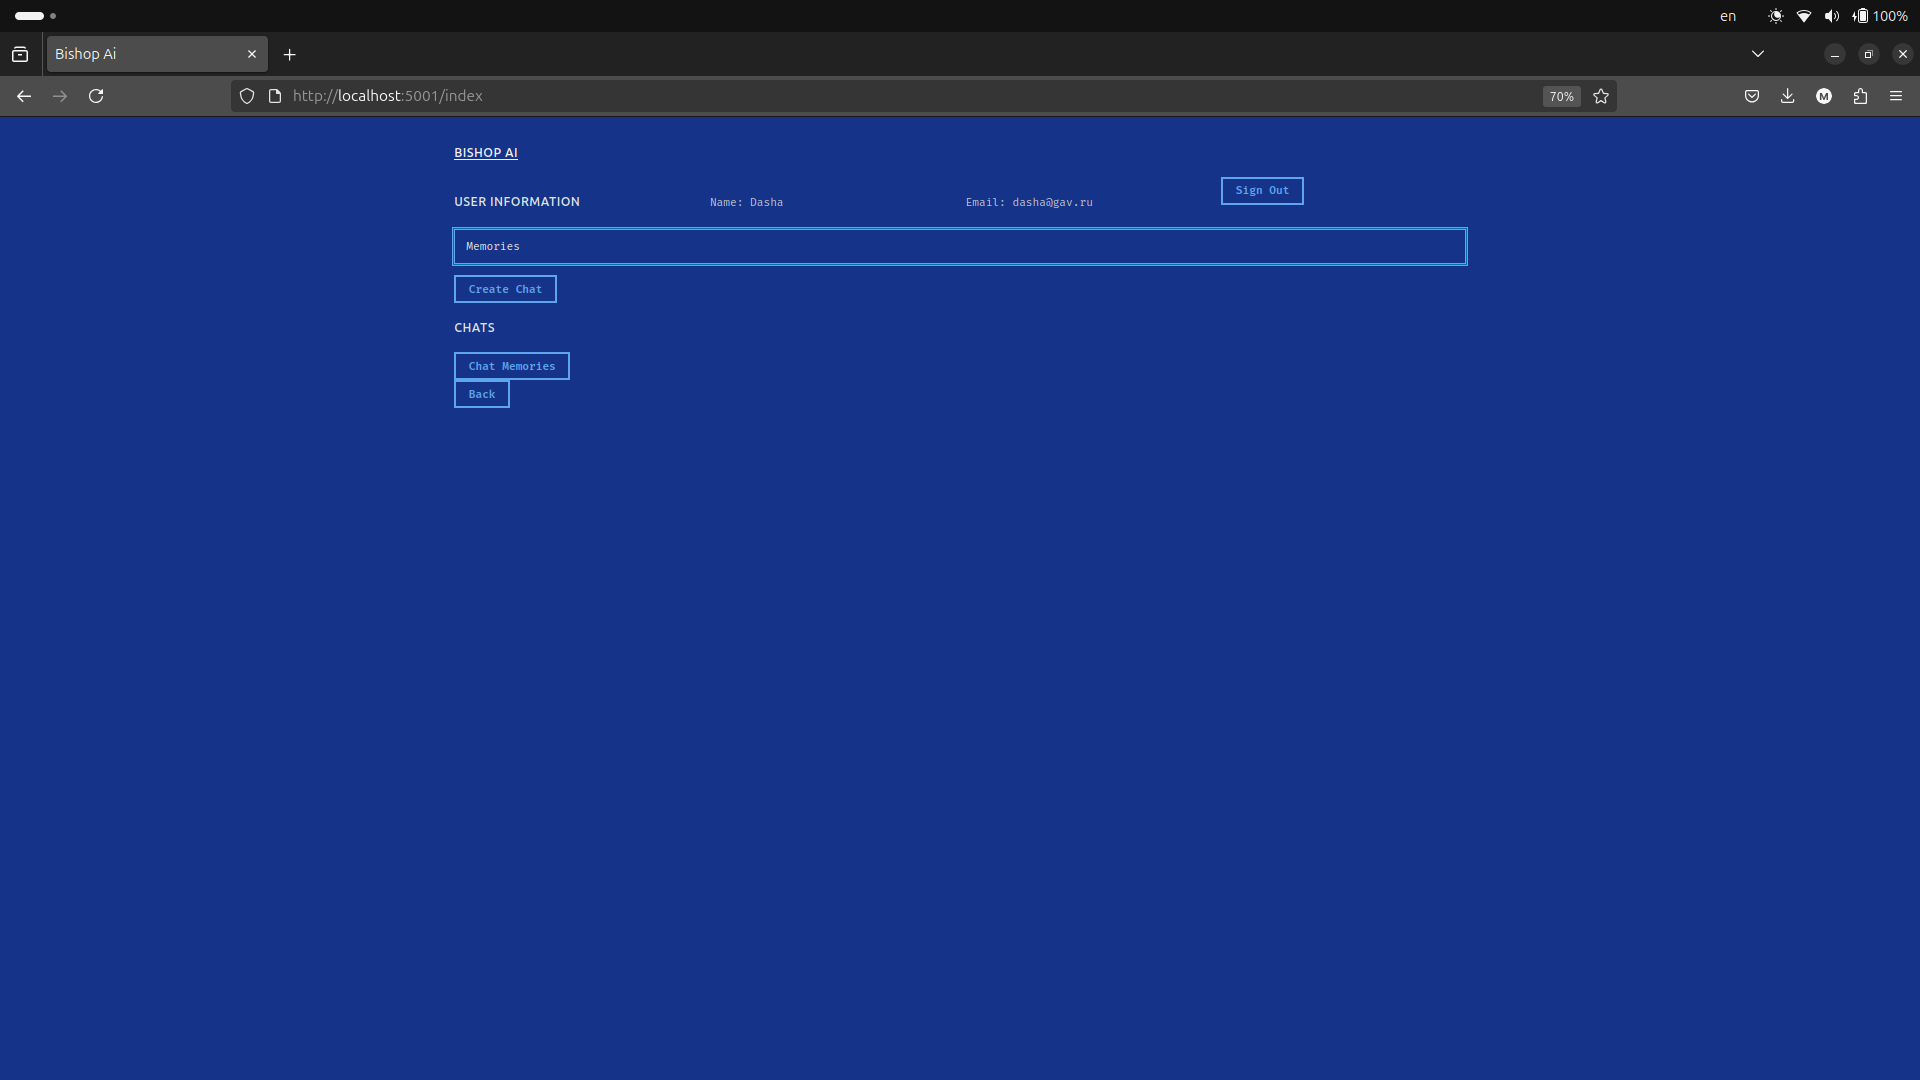
\includegraphics[width=1.0\linewidth]{images/ui/chat1.png}
    \caption{Страница управления чатами}
    \label{fig:ui-page-chat1}
\end{figure}

\begin{figure}
    \centering
    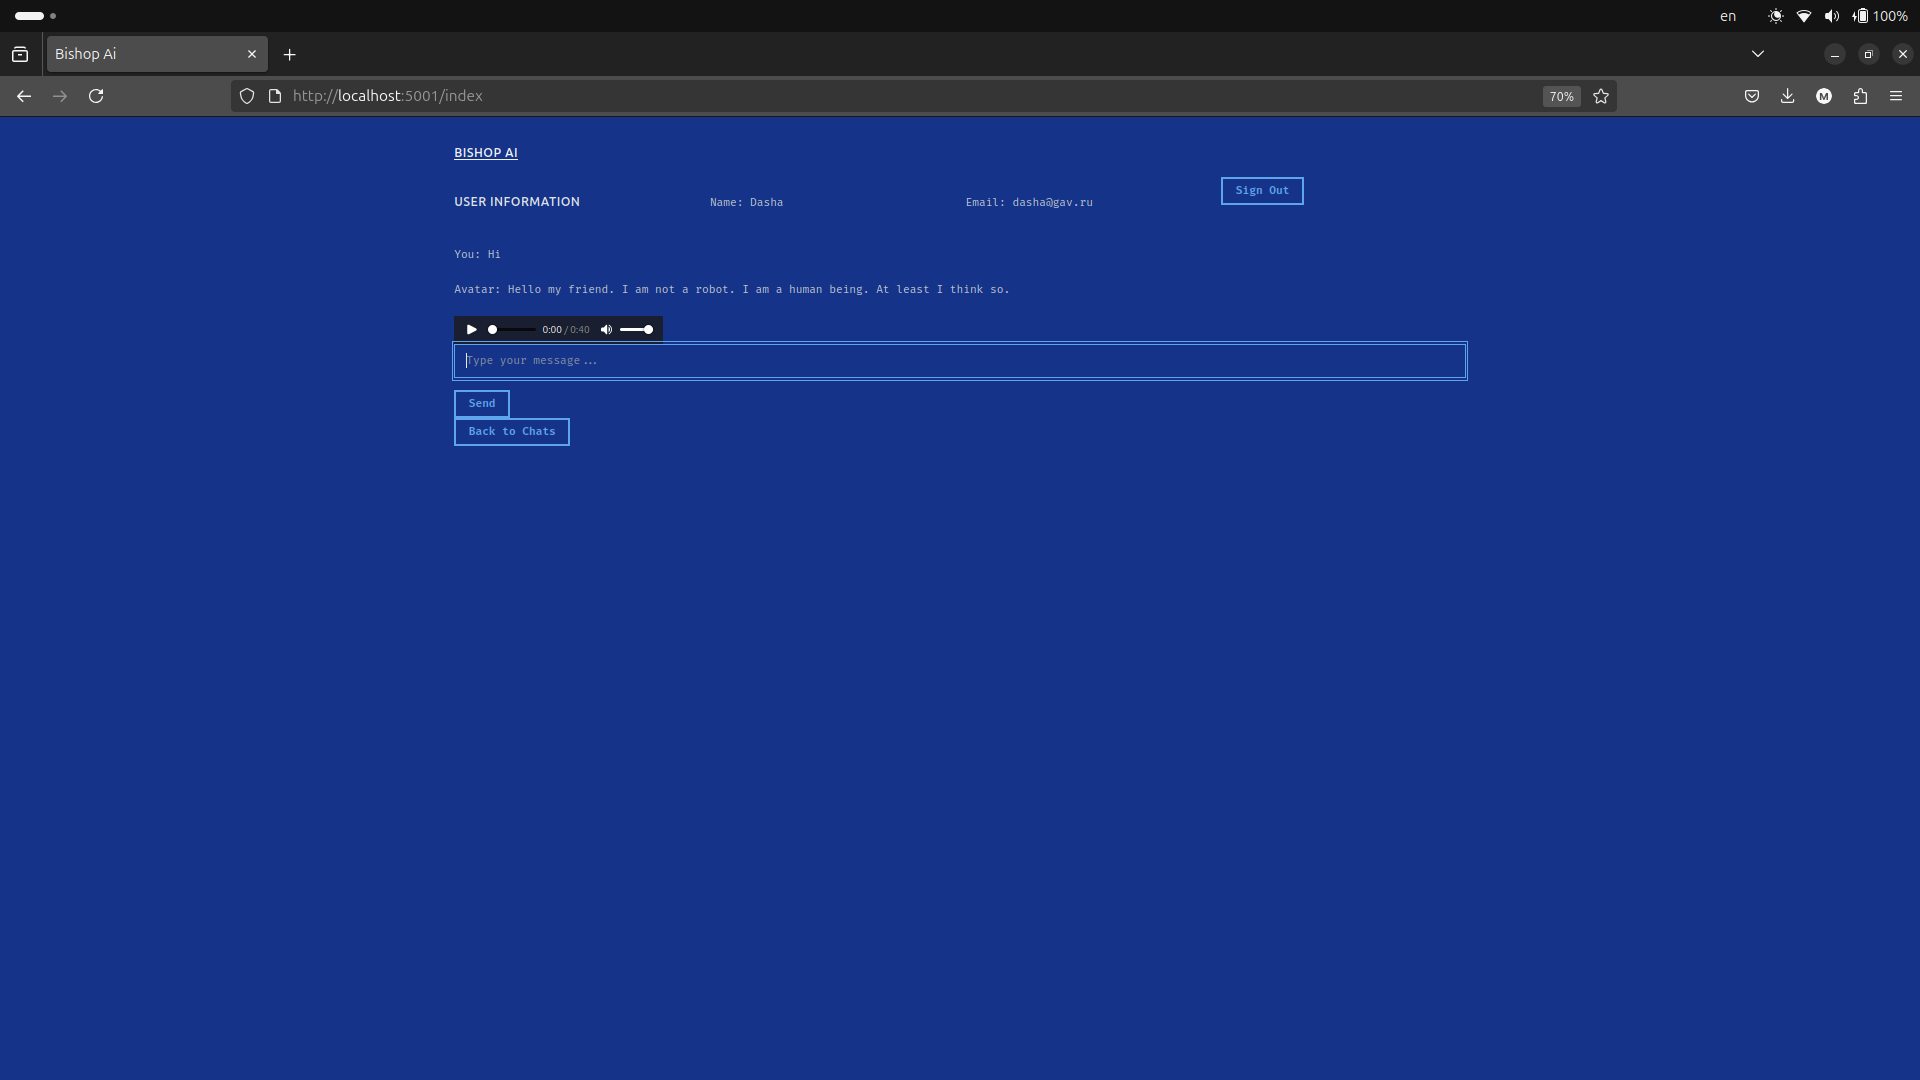
\includegraphics[width=1.0\linewidth]{images/ui/chat2.png}
    \caption{Страница чата}
    \label{fig:ui-page-chat2}
\end{figure}

\begin{figure}
    \centering
    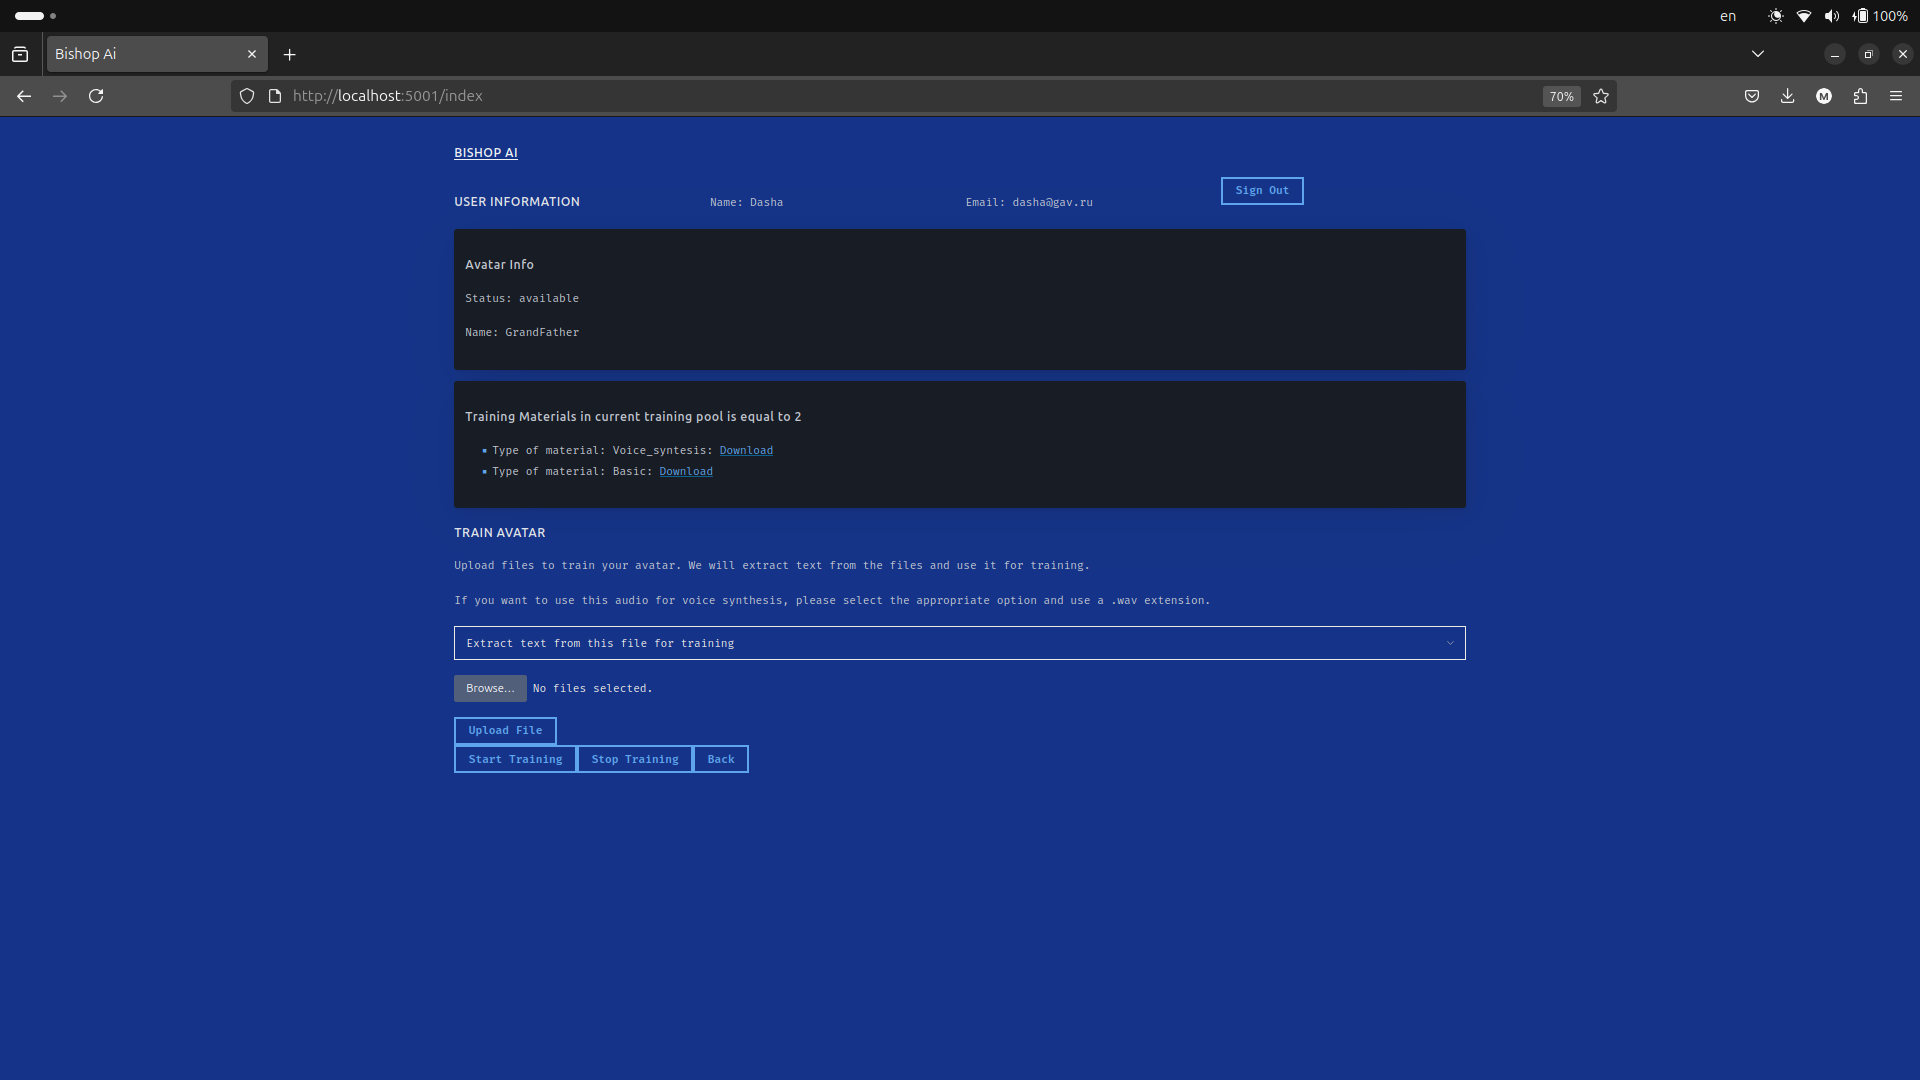
\includegraphics[width=1.0\linewidth]{images/ui/train.png}
    \caption{Интерфейс обучения аватара}
    \label{fig:ui-page-train}
\end{figure}

\chapter{Отчёты о работе сервиса}\label{app:B}

\begin{figure}[h!]
    \centering
    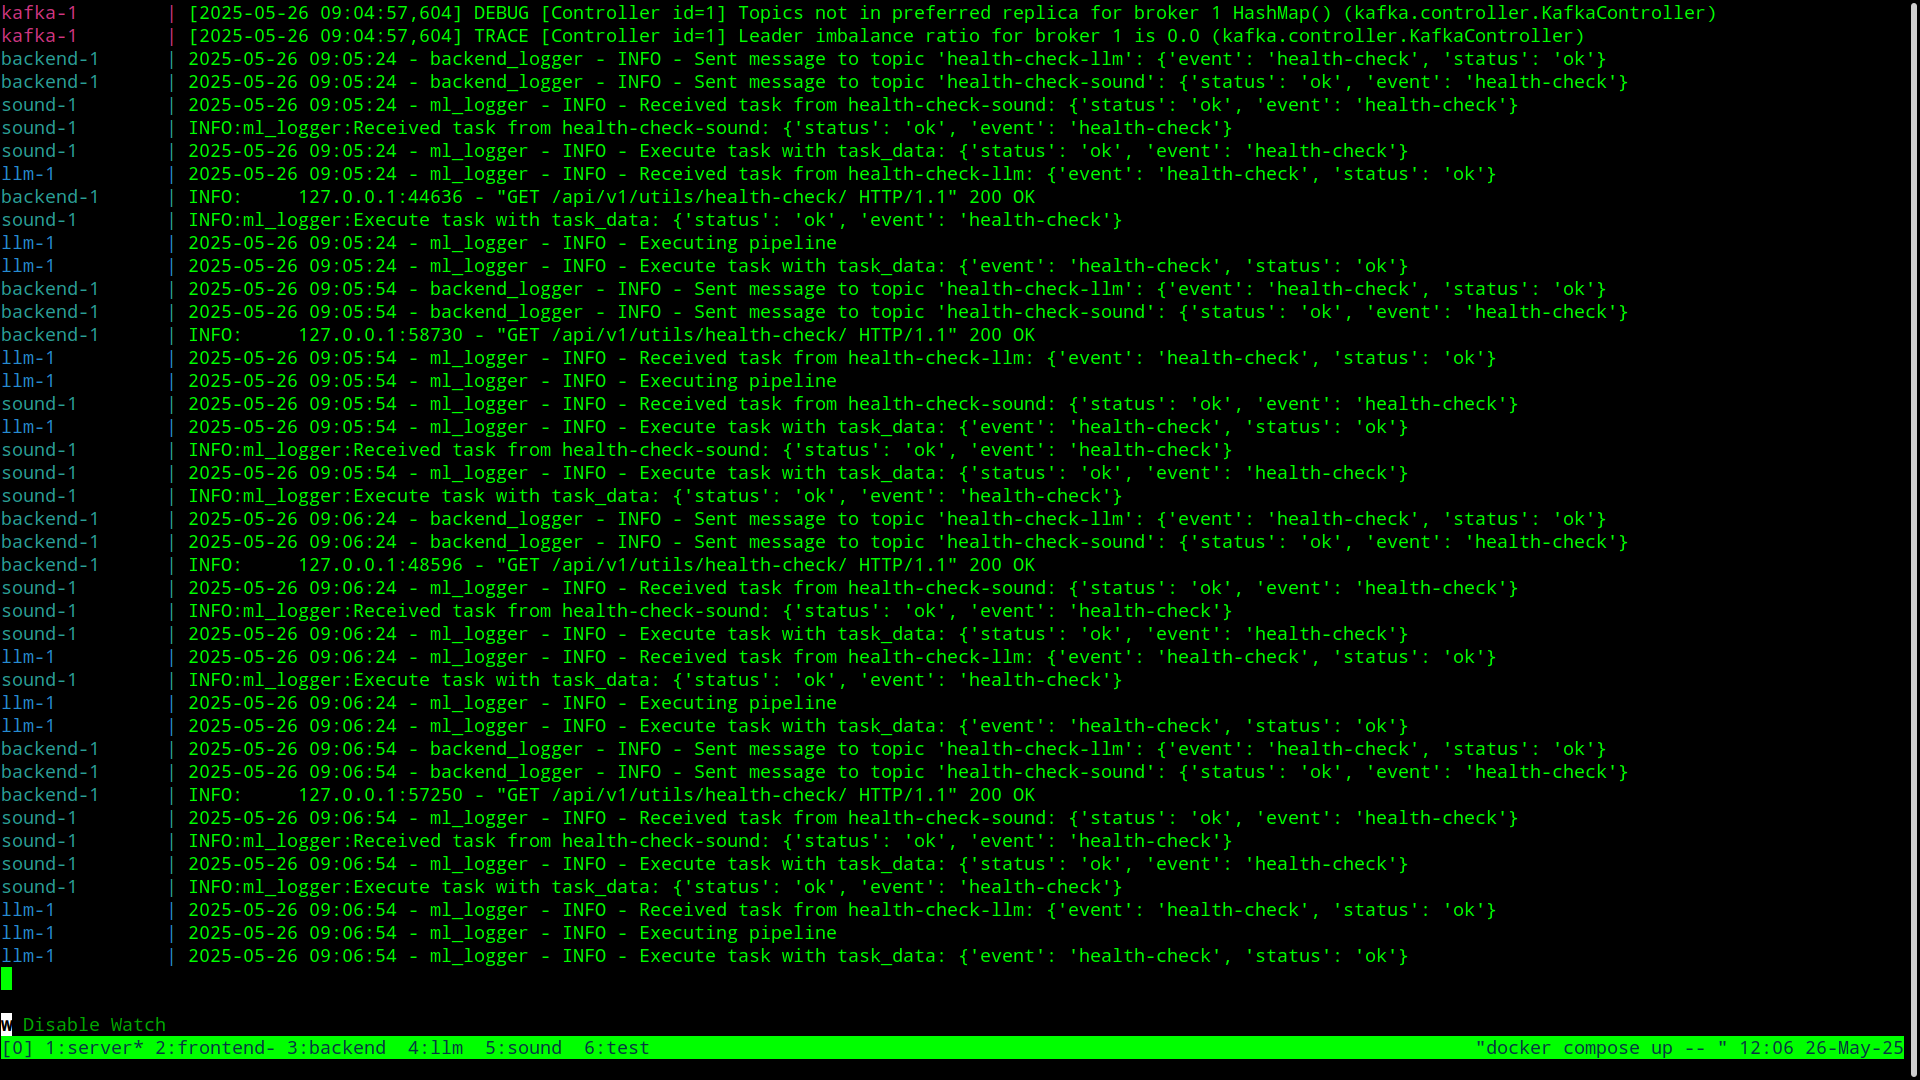
\includegraphics[width=1.0\linewidth]{images/results/health-check.png}
    \caption{Фрагмент логов инициализации системы и периодической проверки состояния доступности системы}
    \label{fig:res-healt-check}
\end{figure}

\begin{figure}
    \centering
    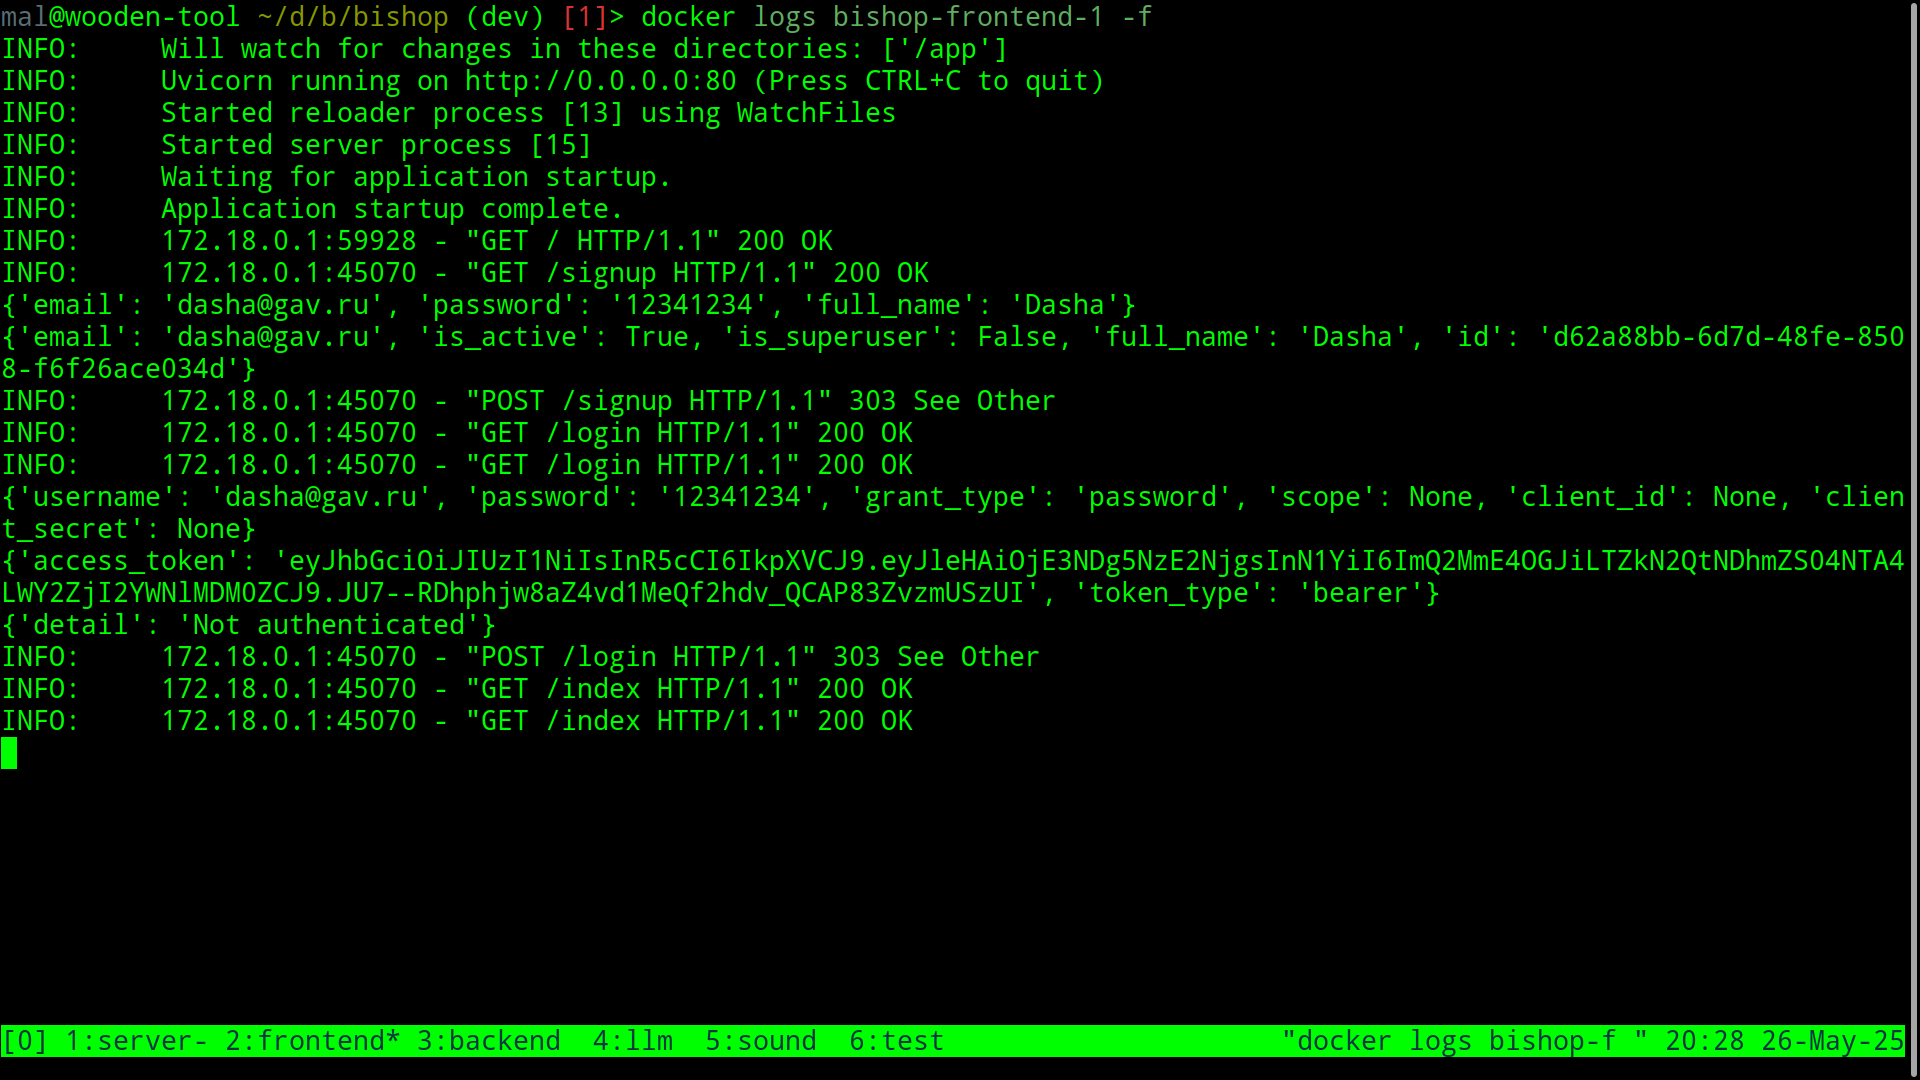
\includegraphics[width=1.0\linewidth]{images/results/signup-login-frontend.png}
    \caption{Регистрация и авторизация пользователя}
    \label{fig:res-signup-login-frontend}
\end{figure}

\begin{figure}
    \centering
    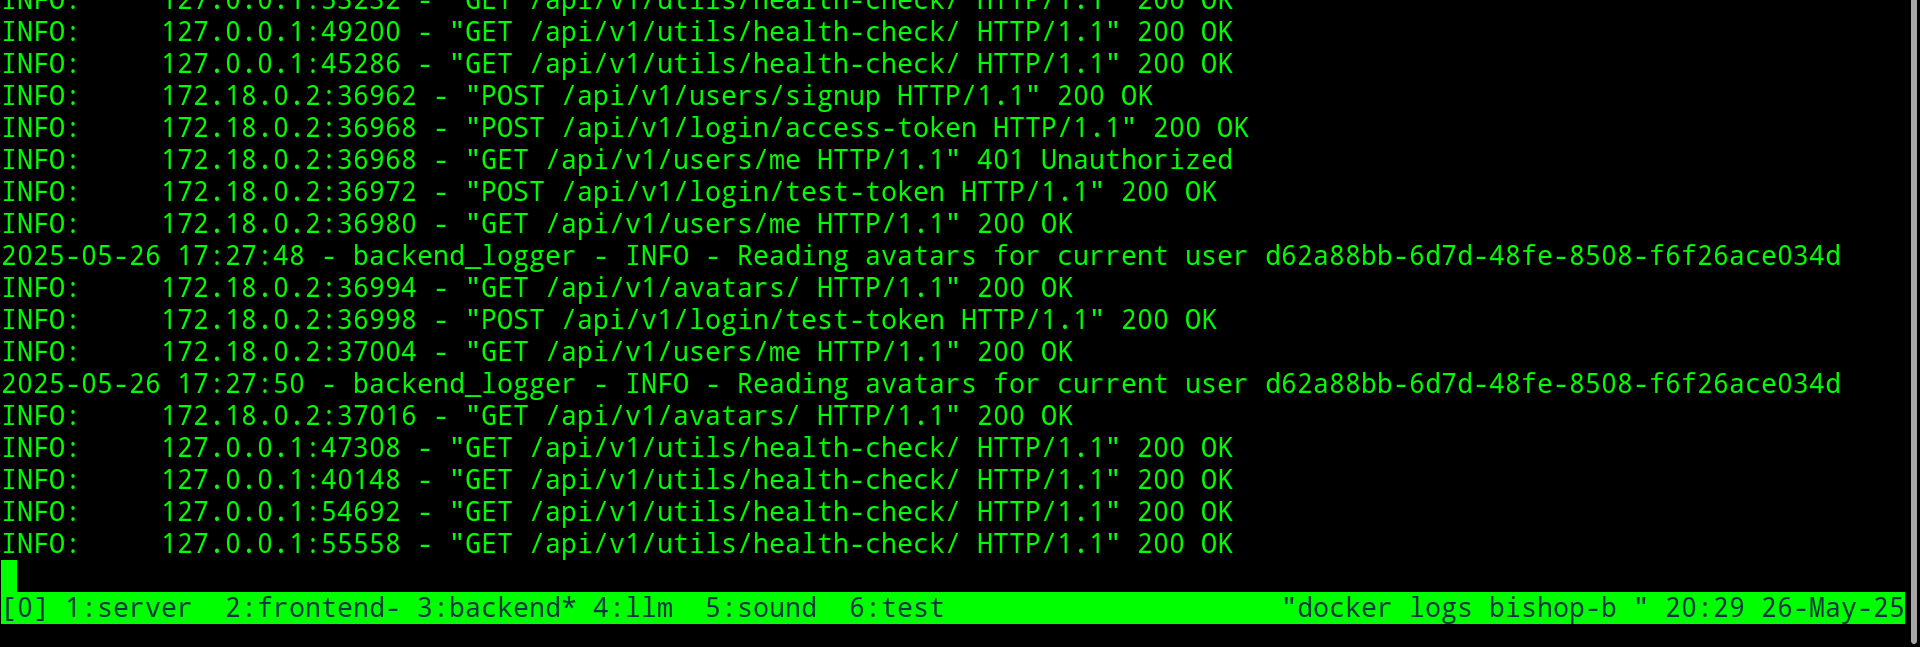
\includegraphics[width=1.0\linewidth]{images/results/signup-login-backend.png}
    \caption{Обработка регистрации и авторизации на стороне backend-сервиса}
    \label{fig:res-signup-login-backend}
\end{figure}

\begin{figure}
    \centering
    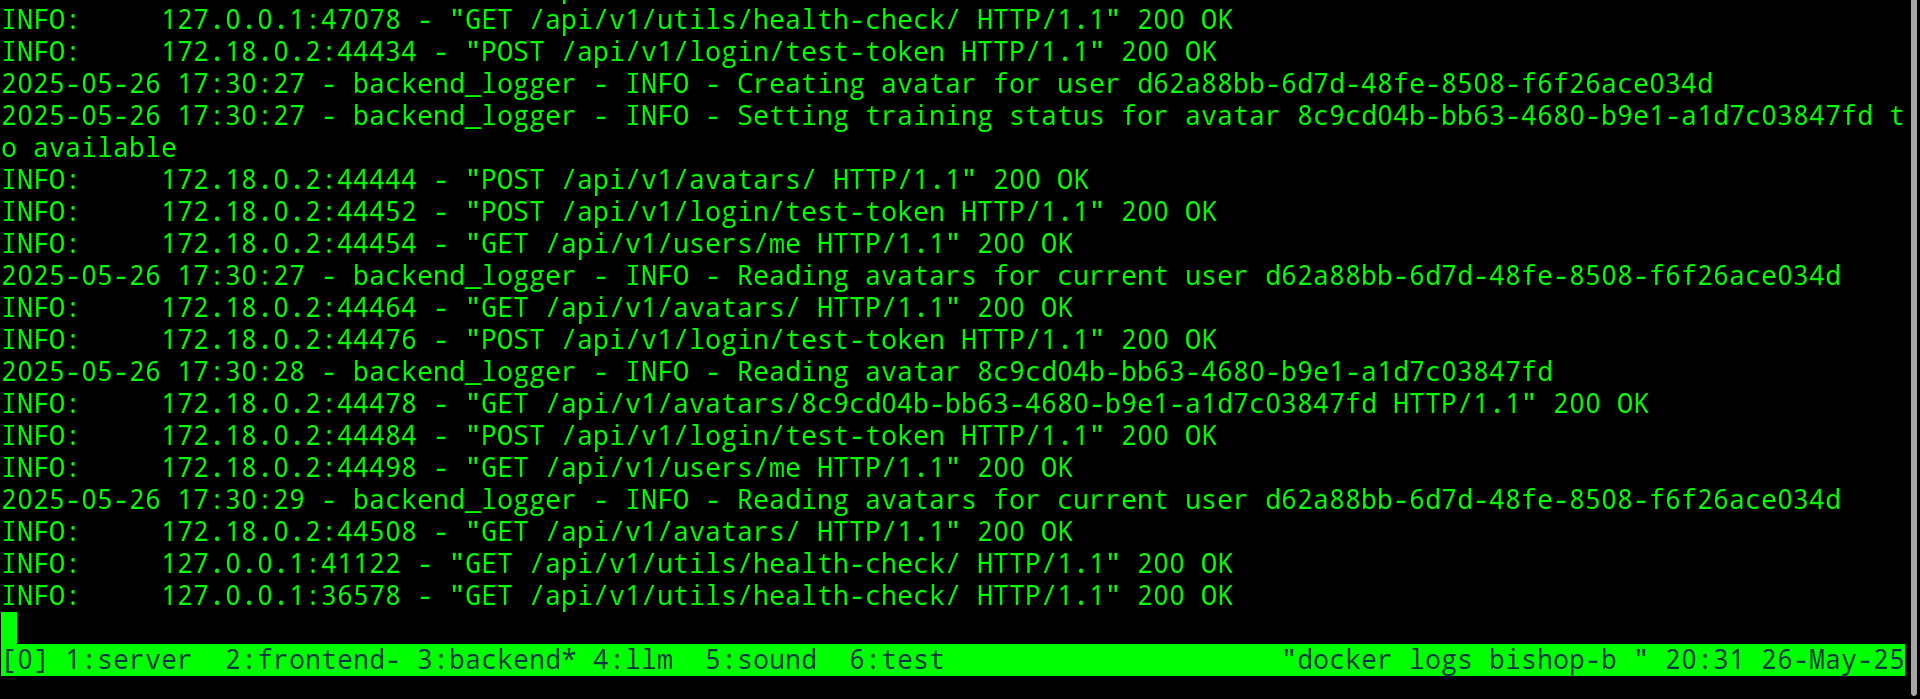
\includegraphics[width=1.0\linewidth]{images/results/bk-create-avatar.png}
    \caption{Создание нового цифрового аватара пользователем}
    \label{fig:res-bk-create-avatar}
\end{figure}

\begin{figure}
    \centering
    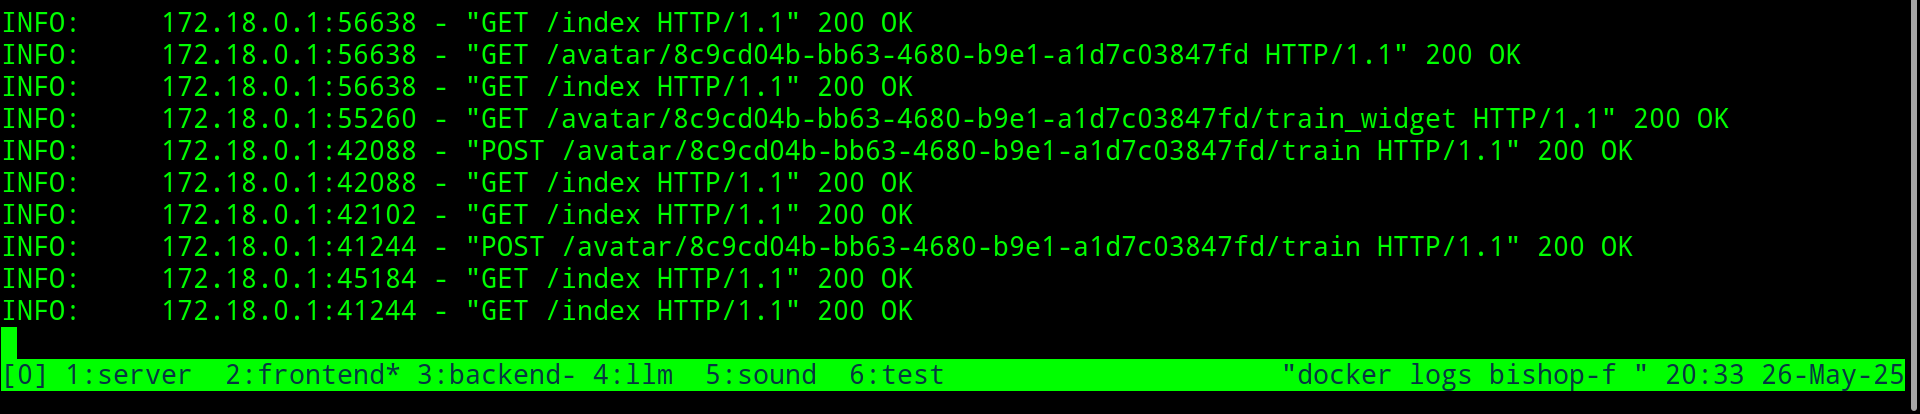
\includegraphics[width=1.0\linewidth]{images/results/fr-upload-materials.png}
    \caption{Загрузка текстовых и аудиофайлов через интерфейс}
    \label{fig:res-fr-upload-materials}
\end{figure}

\begin{figure}
    \centering
    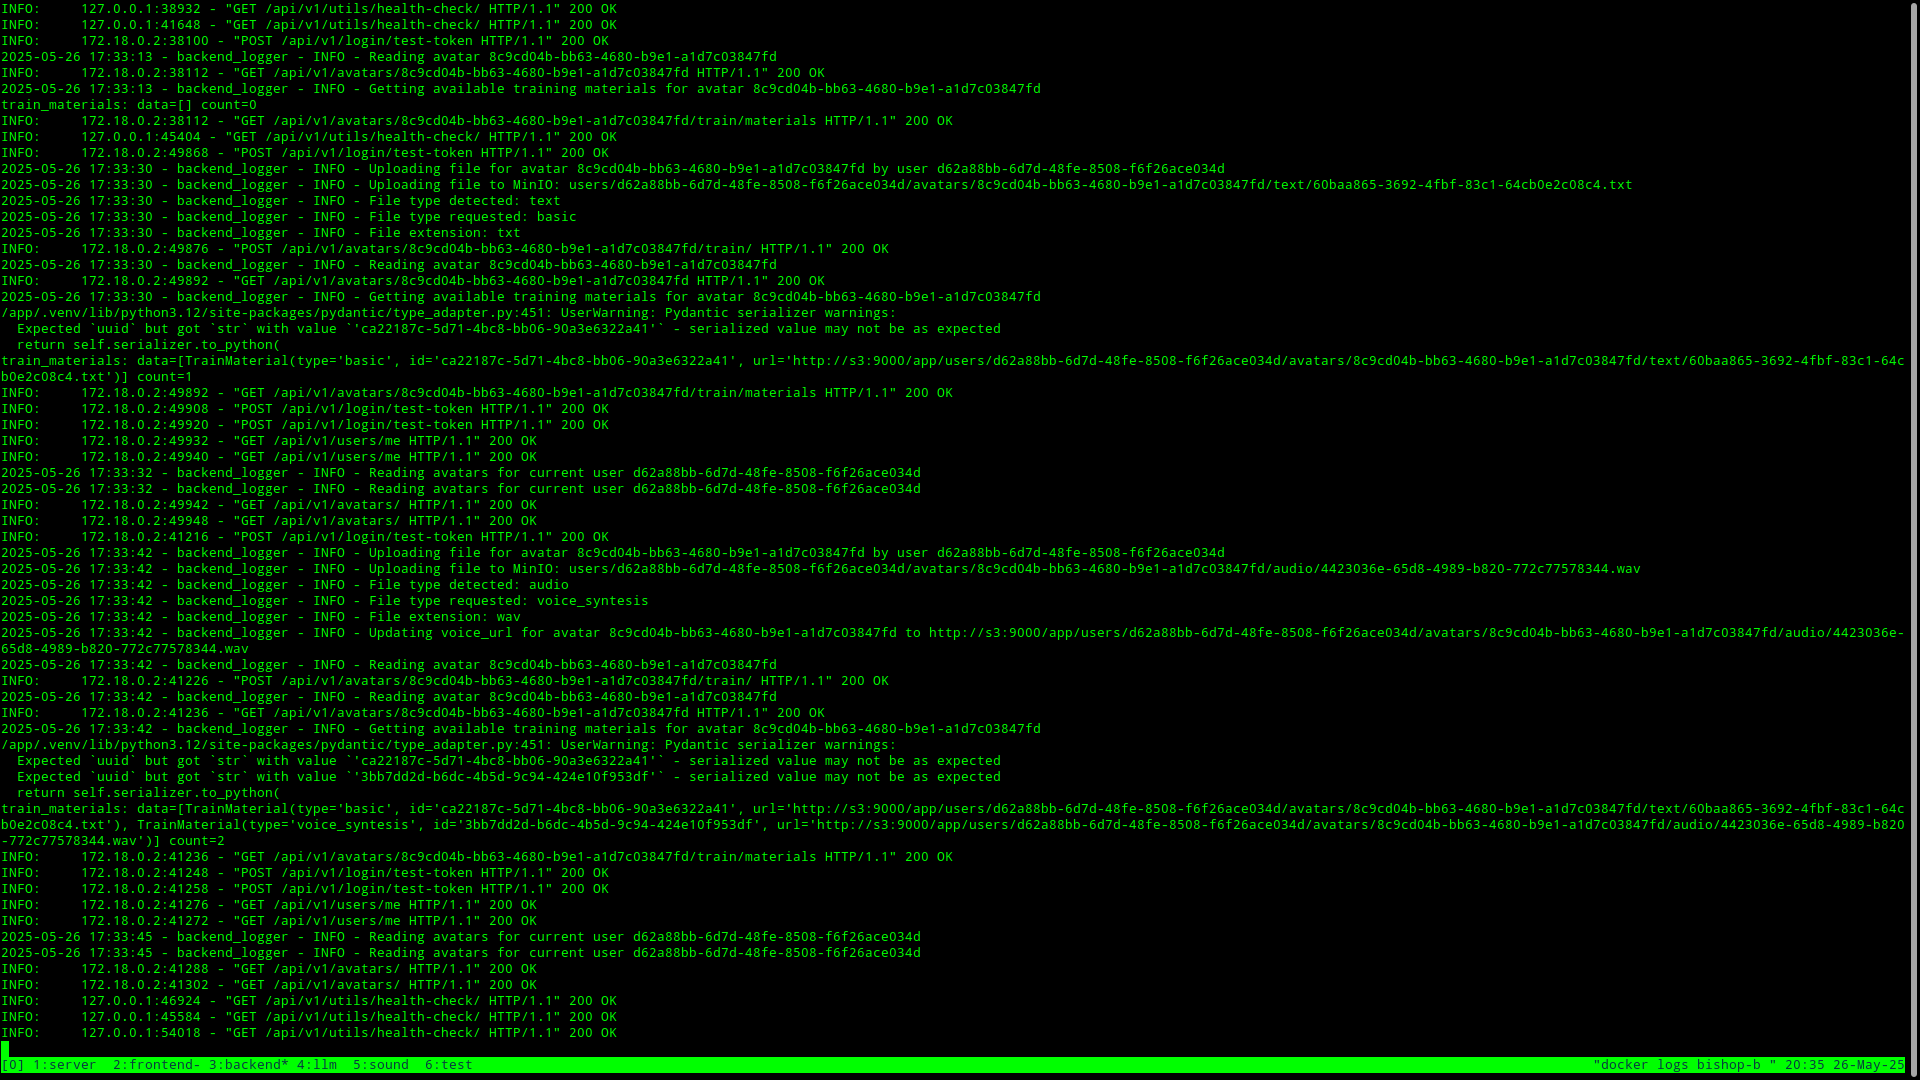
\includegraphics[width=1.0\linewidth]{images/results/bk-upload-materials.png}
    \caption{Фиксация и сохранение обучающих материалов на стороне backend}
    \label{fig:res-bk-upload-materials}
\end{figure}

\begin{figure}
    \centering
    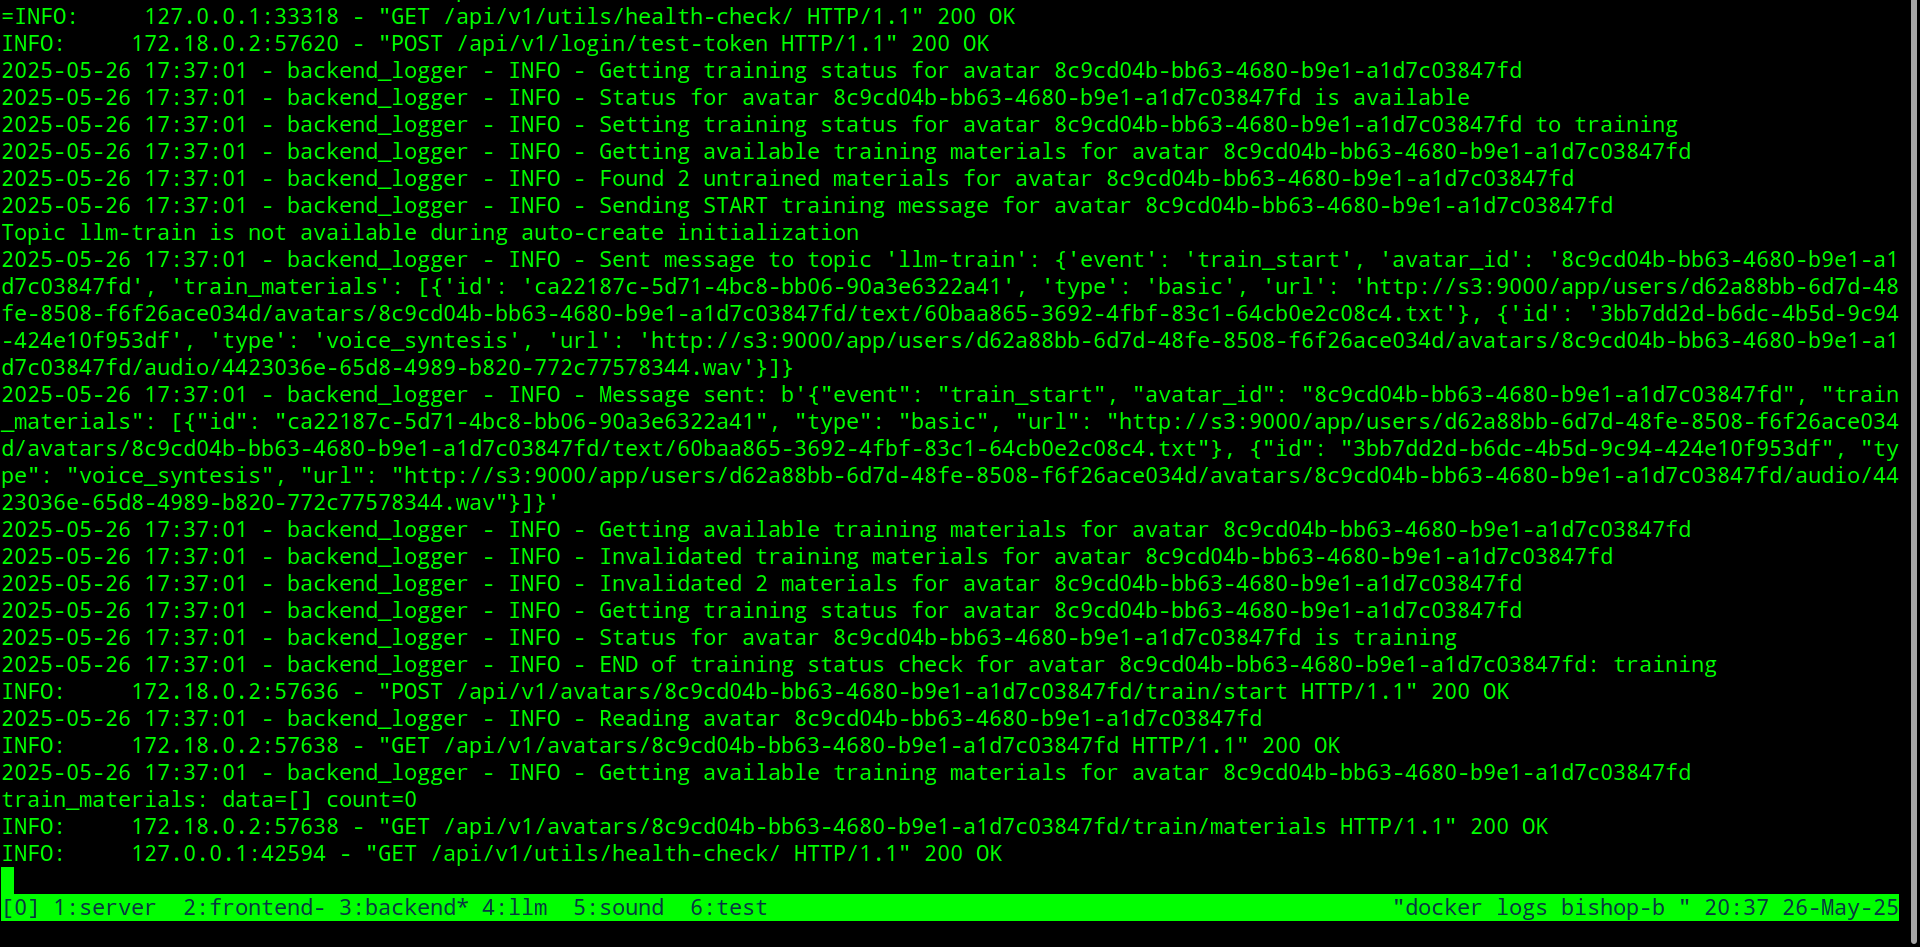
\includegraphics[width=1.0\linewidth]{images/results/bk-start-train.png}
    \caption{Инициация процесса обучения через backend}
    \label{fig:res-bk-start-train}
\end{figure}

\begin{figure}
    \centering
    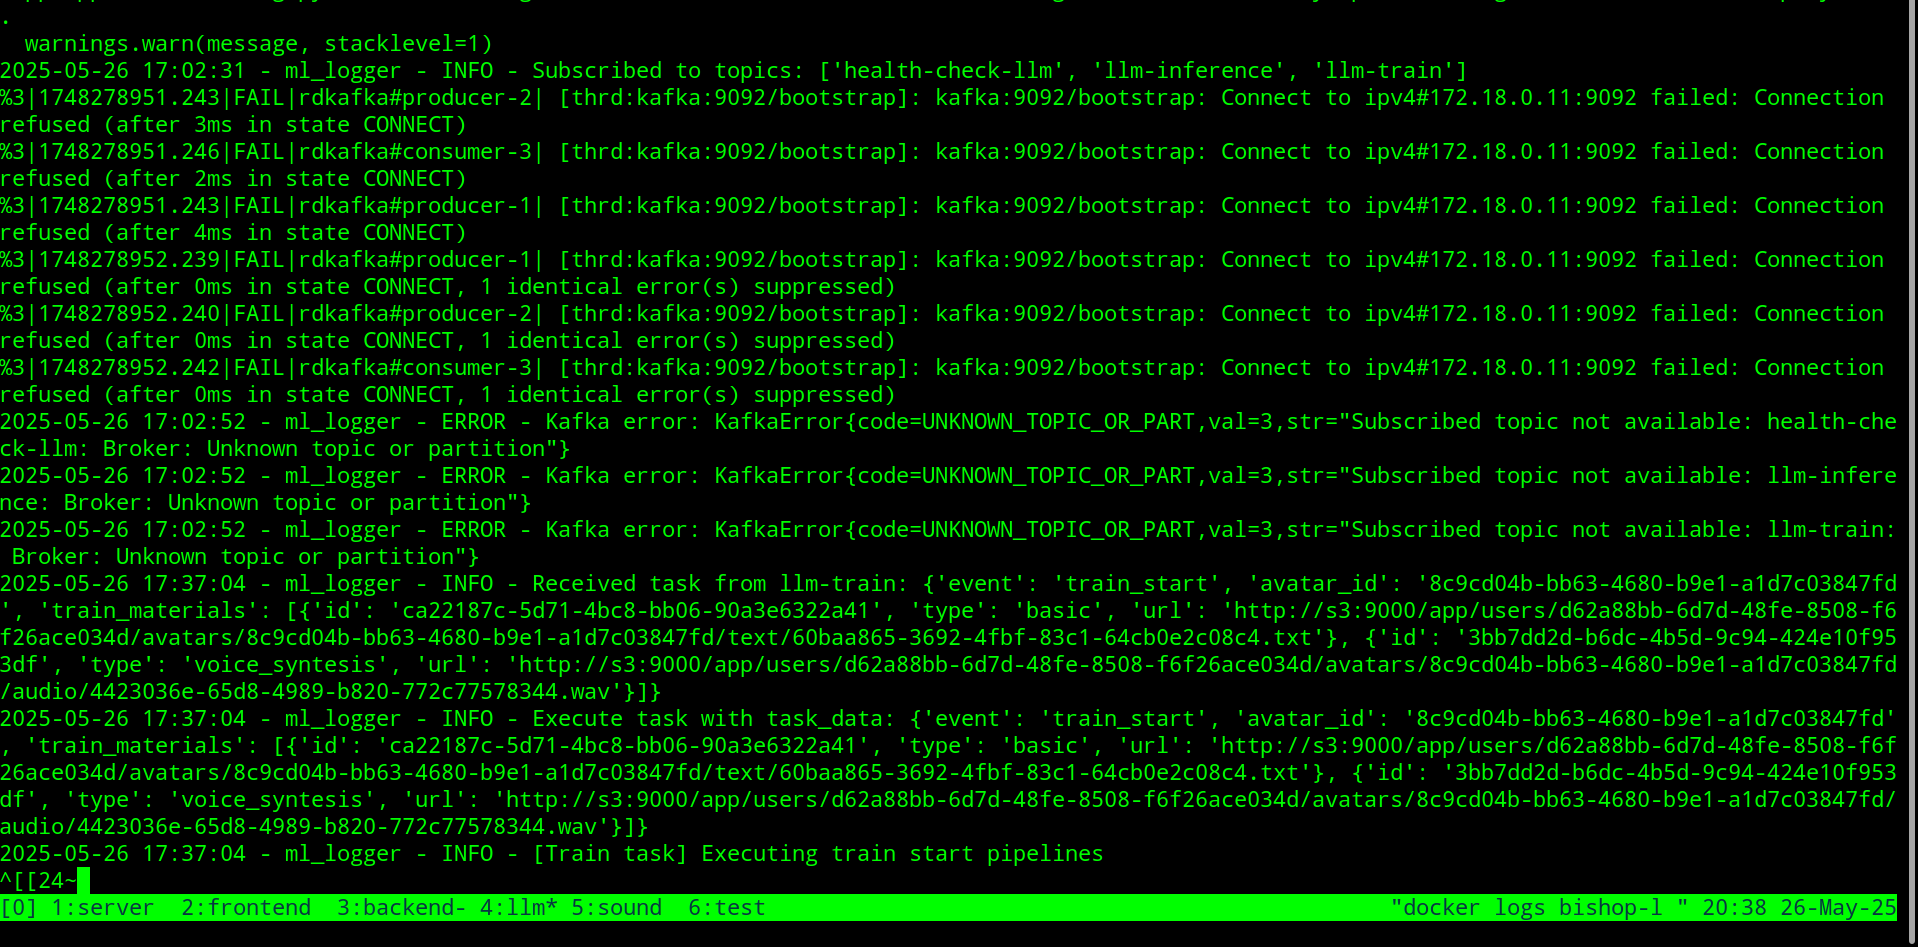
\includegraphics[width=1.0\linewidth]{images/results/llm-start-train.png}
    \caption{Запуск дообучения в модуле генерации текста}
    \label{fig:res-llm-start-train}
\end{figure}

\begin{figure}
    \centering
    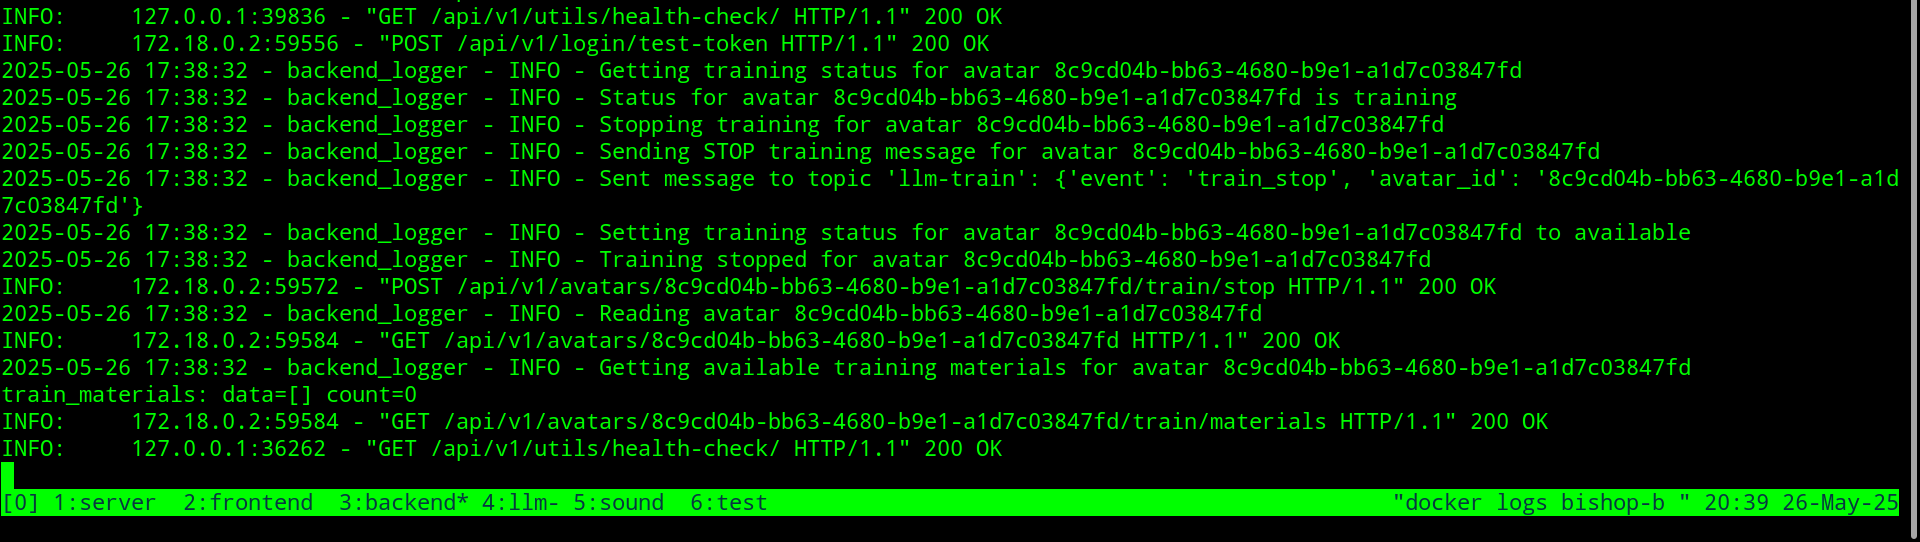
\includegraphics[width=1.0\linewidth]{images/results/bk-stop-train.png}
    \caption{Завершение обучения на стороне backend и обновление статуса}
    \label{fig:res-bk-stop-train}
\end{figure}

\begin{figure}
    \centering
    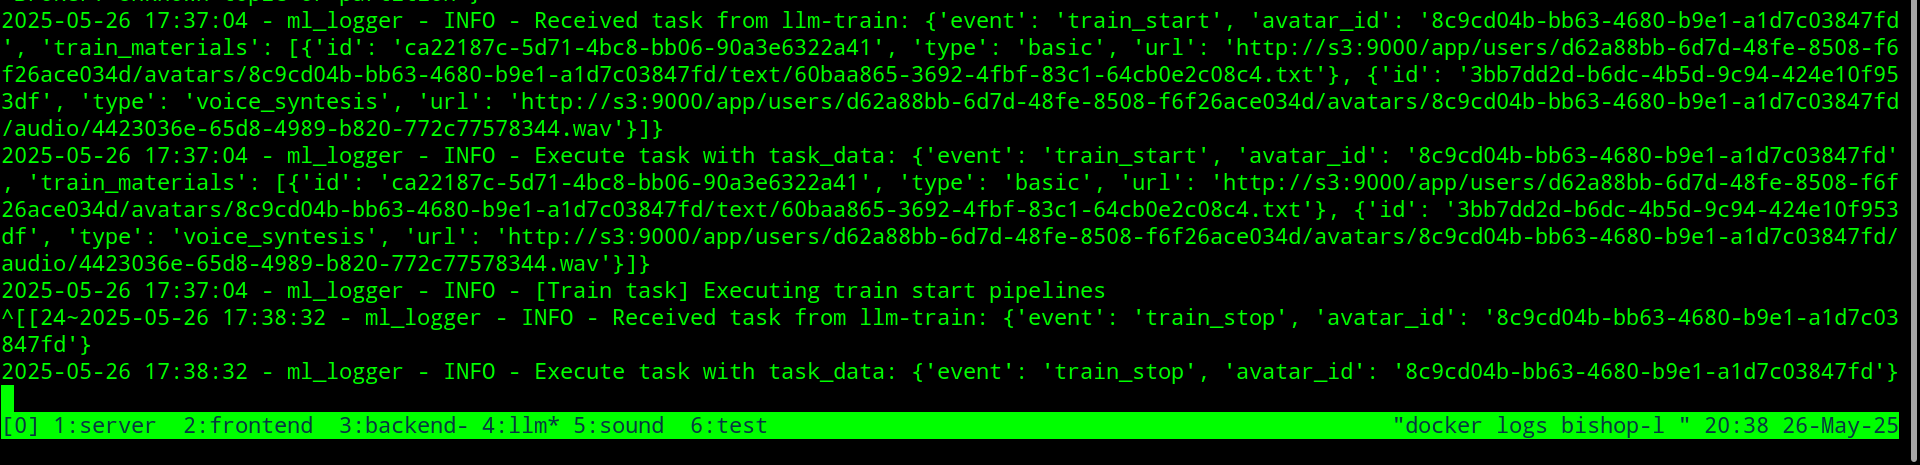
\includegraphics[width=1.0\linewidth]{images/results/llm-stop-train.png}
    \caption{Окончание дообучения модели генерации текста}
    \label{fig:res-llm-stop-train}
\end{figure}

\begin{figure}
    \centering
    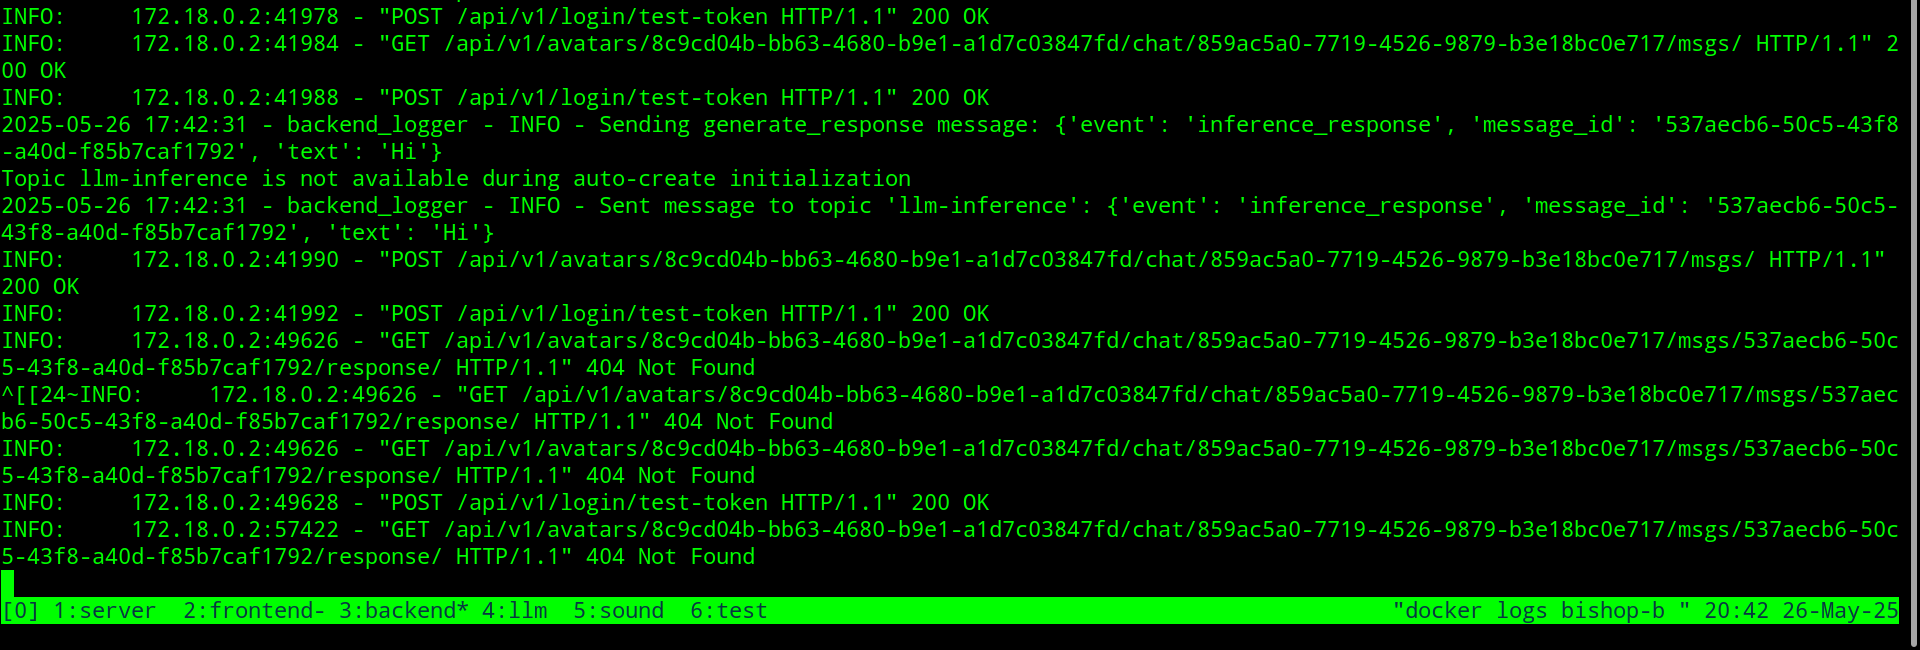
\includegraphics[width=1.0\linewidth]{images/results/bk-start-gen-llm.png}
    \caption{Отправка пользовательского сообщения и генерация текста}
    \label{fig:res-bk-start-gen-llm}
\end{figure}

\begin{figure}
    \centering
    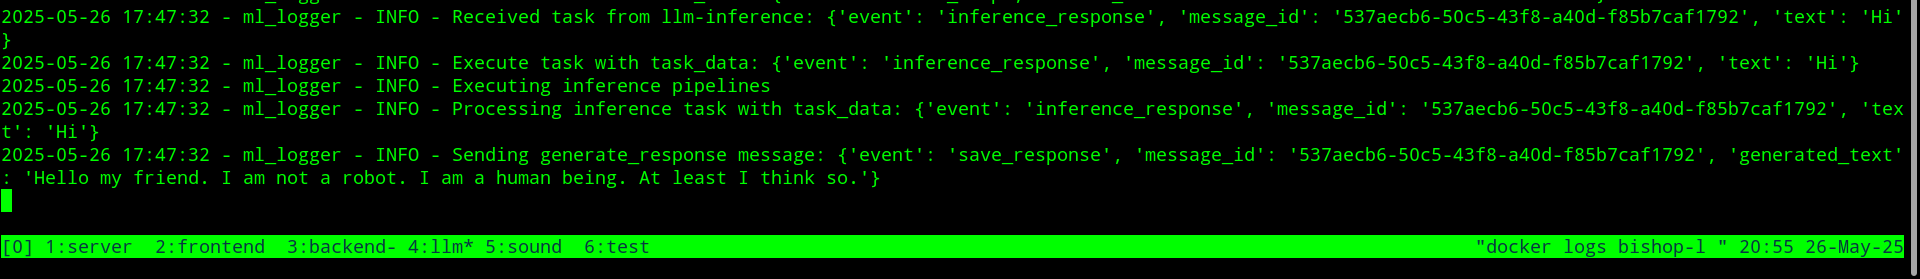
\includegraphics[width=1.0\linewidth]{images/results/llm-inference.png}
    \caption{Генерация ответа llm-моделью по заданному сообщению}
    \label{fig:res-llm-inference}
\end{figure}

\begin{figure}
    \centering
    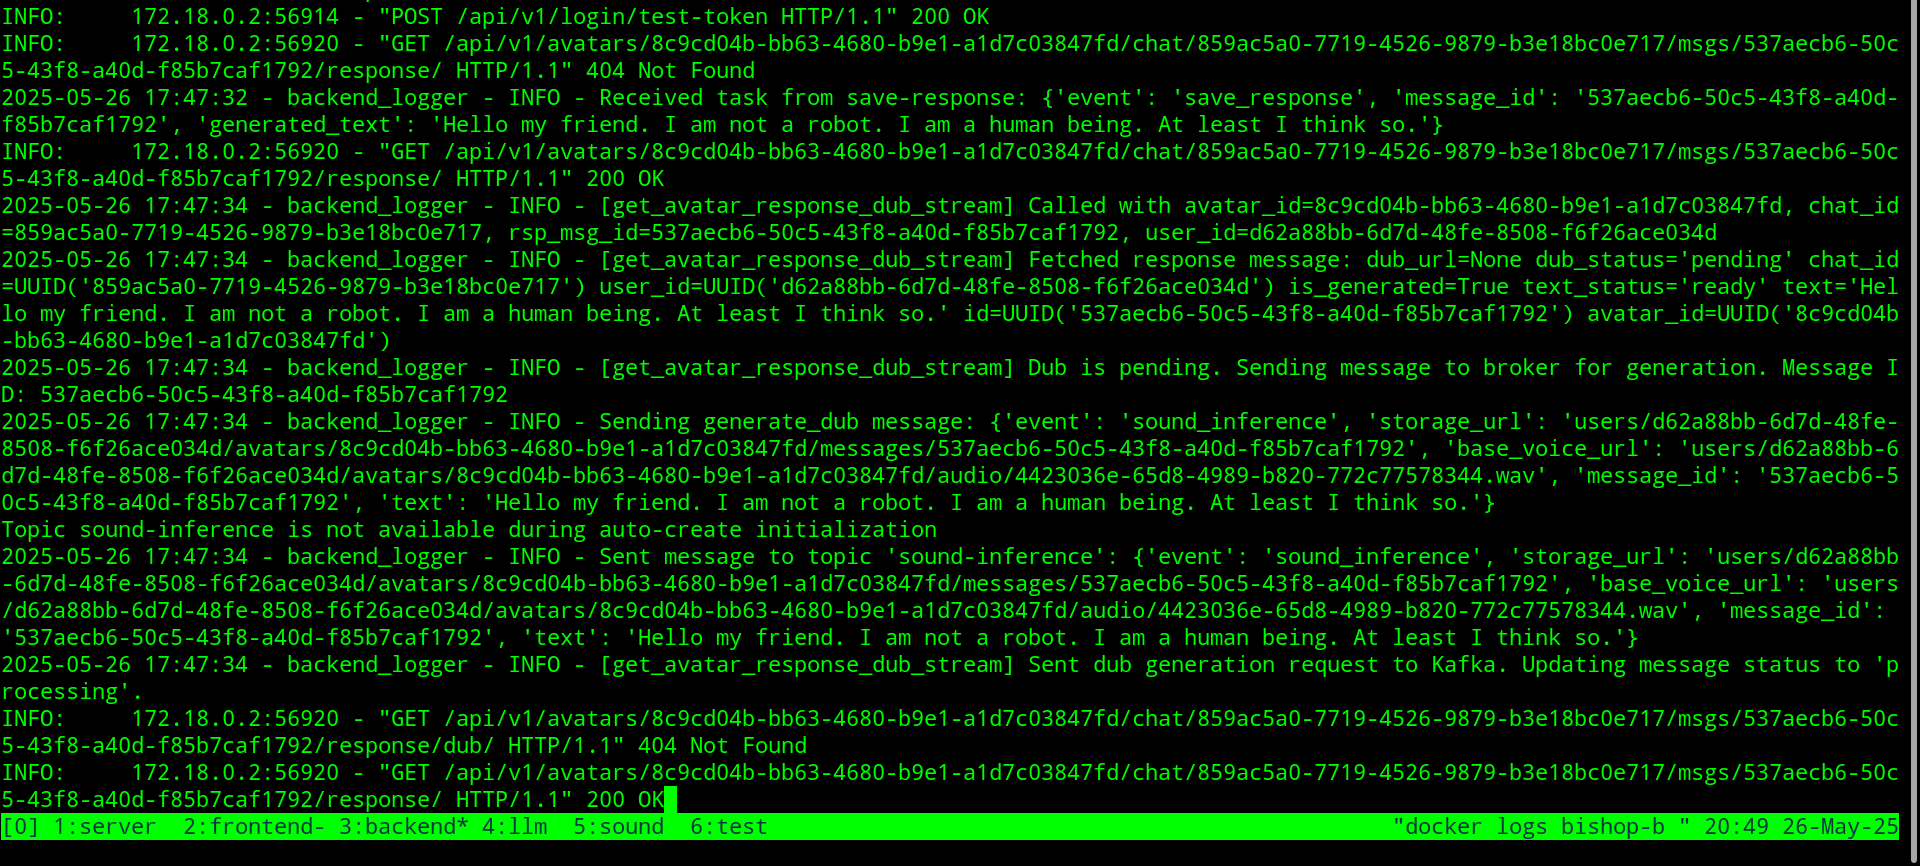
\includegraphics[width=1.0\linewidth]{images/results/bk-middle-gen-llm-done.png}
    \caption{Обработка сгенерированного текста и подготовка к озвучке}
    \label{fig:res-bk-middle-gen-llm-done}
\end{figure}

\begin{figure}
    \centering
    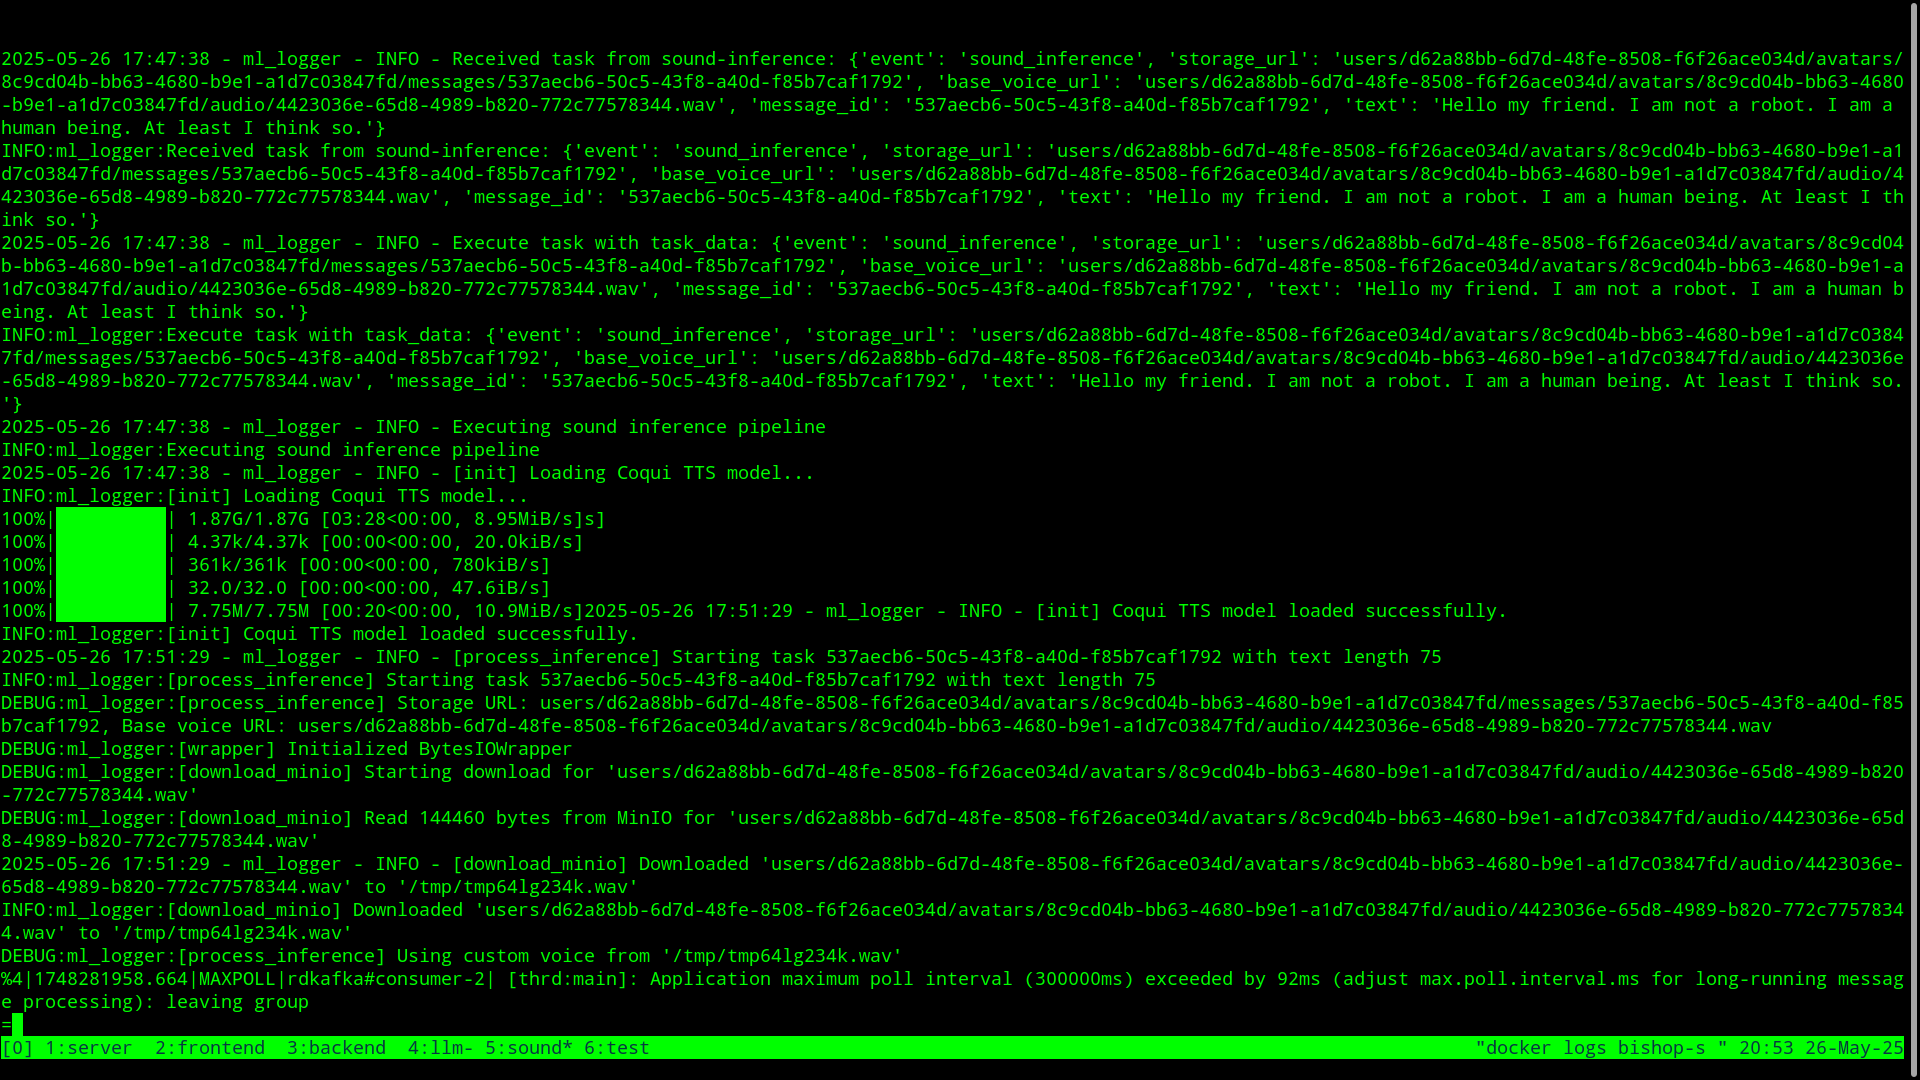
\includegraphics[width=1.0\linewidth]{images/results/sound-inference.png}
    \caption{Генерация аудиофайла на основе текста в сервисе озвучивания}
    \label{fig:res-sound-inference}
\end{figure}

\begin{figure}
    \centering
    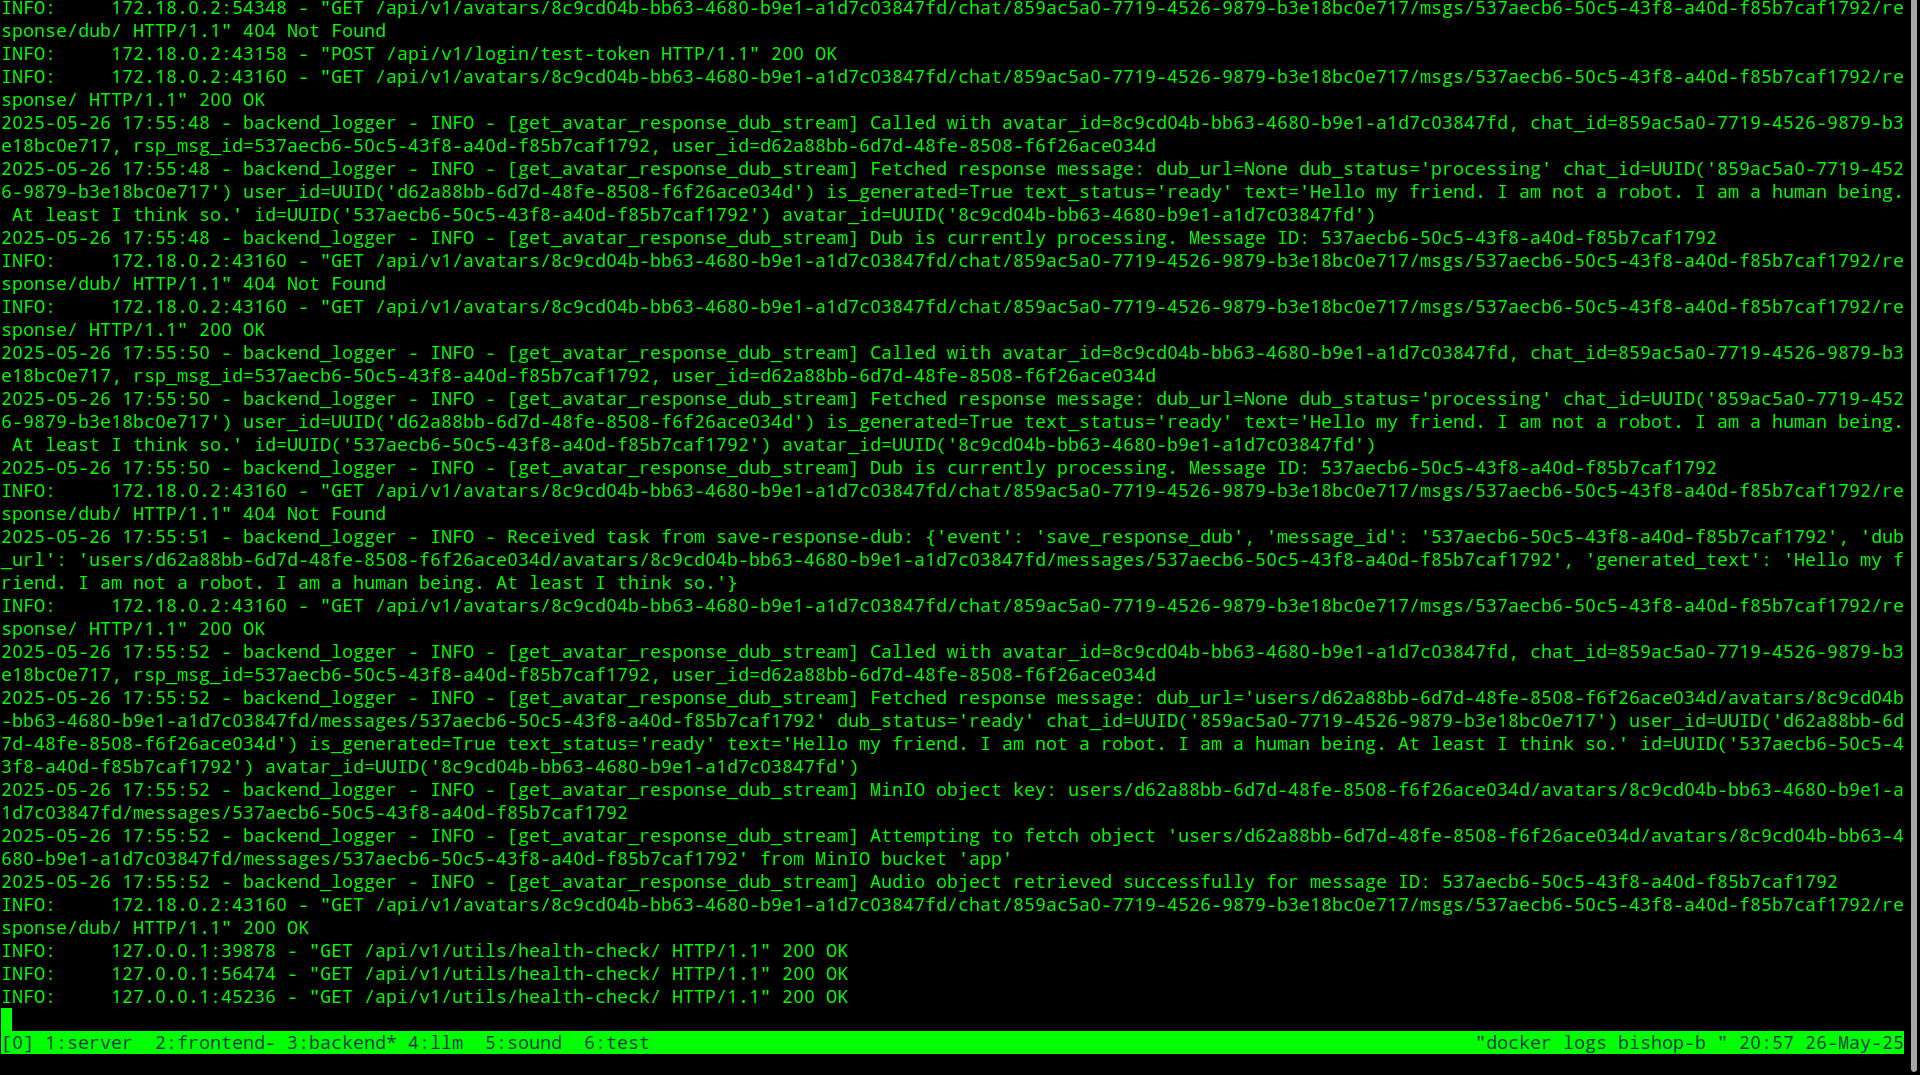
\includegraphics[width=1.0\linewidth]{images/results/bk-end-inference.png}
    \caption{Завершение ответа: возврат текста и аудио пользователю}
    \label{fig:res-bk-end-inference}
\end{figure}